\documentclass[]{article}
\usepackage{lmodern}
\usepackage{amssymb,amsmath}
\usepackage{ifxetex,ifluatex}
\usepackage{fixltx2e} % provides \textsubscript
\ifnum 0\ifxetex 1\fi\ifluatex 1\fi=0 % if pdftex
  \usepackage[T1]{fontenc}
  \usepackage[utf8]{inputenc}
\else % if luatex or xelatex
  \ifxetex
    \usepackage{mathspec}
  \else
    \usepackage{fontspec}
  \fi
  \defaultfontfeatures{Ligatures=TeX,Scale=MatchLowercase}
    \setmainfont[]{Lato}
\fi
% use upquote if available, for straight quotes in verbatim environments
\IfFileExists{upquote.sty}{\usepackage{upquote}}{}
% use microtype if available
\IfFileExists{microtype.sty}{%
\usepackage{microtype}
\UseMicrotypeSet[protrusion]{basicmath} % disable protrusion for tt fonts
}{}
\usepackage[margin=1in]{geometry}
\usepackage{hyperref}
\hypersetup{unicode=true,
            pdftitle={Statistical analysis},
            pdfborder={0 0 0},
            breaklinks=true}
\urlstyle{same}  % don't use monospace font for urls
\usepackage{color}
\usepackage{fancyvrb}
\newcommand{\VerbBar}{|}
\newcommand{\VERB}{\Verb[commandchars=\\\{\}]}
\DefineVerbatimEnvironment{Highlighting}{Verbatim}{commandchars=\\\{\}}
% Add ',fontsize=\small' for more characters per line
\usepackage{framed}
\definecolor{shadecolor}{RGB}{248,248,248}
\newenvironment{Shaded}{\begin{snugshade}}{\end{snugshade}}
\newcommand{\AlertTok}[1]{\textcolor[rgb]{0.94,0.16,0.16}{#1}}
\newcommand{\AnnotationTok}[1]{\textcolor[rgb]{0.56,0.35,0.01}{\textbf{\textit{#1}}}}
\newcommand{\AttributeTok}[1]{\textcolor[rgb]{0.77,0.63,0.00}{#1}}
\newcommand{\BaseNTok}[1]{\textcolor[rgb]{0.00,0.00,0.81}{#1}}
\newcommand{\BuiltInTok}[1]{#1}
\newcommand{\CharTok}[1]{\textcolor[rgb]{0.31,0.60,0.02}{#1}}
\newcommand{\CommentTok}[1]{\textcolor[rgb]{0.56,0.35,0.01}{\textit{#1}}}
\newcommand{\CommentVarTok}[1]{\textcolor[rgb]{0.56,0.35,0.01}{\textbf{\textit{#1}}}}
\newcommand{\ConstantTok}[1]{\textcolor[rgb]{0.00,0.00,0.00}{#1}}
\newcommand{\ControlFlowTok}[1]{\textcolor[rgb]{0.13,0.29,0.53}{\textbf{#1}}}
\newcommand{\DataTypeTok}[1]{\textcolor[rgb]{0.13,0.29,0.53}{#1}}
\newcommand{\DecValTok}[1]{\textcolor[rgb]{0.00,0.00,0.81}{#1}}
\newcommand{\DocumentationTok}[1]{\textcolor[rgb]{0.56,0.35,0.01}{\textbf{\textit{#1}}}}
\newcommand{\ErrorTok}[1]{\textcolor[rgb]{0.64,0.00,0.00}{\textbf{#1}}}
\newcommand{\ExtensionTok}[1]{#1}
\newcommand{\FloatTok}[1]{\textcolor[rgb]{0.00,0.00,0.81}{#1}}
\newcommand{\FunctionTok}[1]{\textcolor[rgb]{0.00,0.00,0.00}{#1}}
\newcommand{\ImportTok}[1]{#1}
\newcommand{\InformationTok}[1]{\textcolor[rgb]{0.56,0.35,0.01}{\textbf{\textit{#1}}}}
\newcommand{\KeywordTok}[1]{\textcolor[rgb]{0.13,0.29,0.53}{\textbf{#1}}}
\newcommand{\NormalTok}[1]{#1}
\newcommand{\OperatorTok}[1]{\textcolor[rgb]{0.81,0.36,0.00}{\textbf{#1}}}
\newcommand{\OtherTok}[1]{\textcolor[rgb]{0.56,0.35,0.01}{#1}}
\newcommand{\PreprocessorTok}[1]{\textcolor[rgb]{0.56,0.35,0.01}{\textit{#1}}}
\newcommand{\RegionMarkerTok}[1]{#1}
\newcommand{\SpecialCharTok}[1]{\textcolor[rgb]{0.00,0.00,0.00}{#1}}
\newcommand{\SpecialStringTok}[1]{\textcolor[rgb]{0.31,0.60,0.02}{#1}}
\newcommand{\StringTok}[1]{\textcolor[rgb]{0.31,0.60,0.02}{#1}}
\newcommand{\VariableTok}[1]{\textcolor[rgb]{0.00,0.00,0.00}{#1}}
\newcommand{\VerbatimStringTok}[1]{\textcolor[rgb]{0.31,0.60,0.02}{#1}}
\newcommand{\WarningTok}[1]{\textcolor[rgb]{0.56,0.35,0.01}{\textbf{\textit{#1}}}}
\usepackage{graphicx,grffile}
\makeatletter
\def\maxwidth{\ifdim\Gin@nat@width>\linewidth\linewidth\else\Gin@nat@width\fi}
\def\maxheight{\ifdim\Gin@nat@height>\textheight\textheight\else\Gin@nat@height\fi}
\makeatother
% Scale images if necessary, so that they will not overflow the page
% margins by default, and it is still possible to overwrite the defaults
% using explicit options in \includegraphics[width, height, ...]{}
\setkeys{Gin}{width=\maxwidth,height=\maxheight,keepaspectratio}
\IfFileExists{parskip.sty}{%
\usepackage{parskip}
}{% else
\setlength{\parindent}{0pt}
\setlength{\parskip}{6pt plus 2pt minus 1pt}
}
\setlength{\emergencystretch}{3em}  % prevent overfull lines
\providecommand{\tightlist}{%
  \setlength{\itemsep}{0pt}\setlength{\parskip}{0pt}}
\setcounter{secnumdepth}{5}
% Redefines (sub)paragraphs to behave more like sections
\ifx\paragraph\undefined\else
\let\oldparagraph\paragraph
\renewcommand{\paragraph}[1]{\oldparagraph{#1}\mbox{}}
\fi
\ifx\subparagraph\undefined\else
\let\oldsubparagraph\subparagraph
\renewcommand{\subparagraph}[1]{\oldsubparagraph{#1}\mbox{}}
\fi

%%% Use protect on footnotes to avoid problems with footnotes in titles
\let\rmarkdownfootnote\footnote%
\def\footnote{\protect\rmarkdownfootnote}

%%% Change title format to be more compact
\usepackage{titling}

% Create subtitle command for use in maketitle
\providecommand{\subtitle}[1]{
  \posttitle{
    \begin{center}\large#1\end{center}
    }
}

\setlength{\droptitle}{-2em}

  \title{Statistical analysis}
    \pretitle{\vspace{\droptitle}\centering\huge}
  \posttitle{\par}
    \author{}
    \preauthor{}\postauthor{}
    \date{}
    \predate{}\postdate{}
  

\begin{document}
\maketitle

\hypertarget{read-data}{%
\section{Read data}\label{read-data}}

These chunks read the data and processes it for analysis.

The following reads \texttt{gestures.csv} and \texttt{utterances.csv}
into \texttt{gesture\_tot} and \texttt{utterances\_tot}.
\texttt{gestures\_tot} has time series data of infant gestures and
maternal Contingent Talks at 10, 11, and 12 months.
\texttt{utterance\_tot} has time series data of maternal utterances at
10, 11, and 12 months. Data is aggregated from the two experimental
activities.

\begin{Shaded}
\begin{Highlighting}[]
\NormalTok{gestures <-}\StringTok{ }\KeywordTok{read_csv}\NormalTok{(}\StringTok{"./data/gestures.csv"}\NormalTok{)}

\NormalTok{gestures_tot <-}\StringTok{ }\NormalTok{gestures }\OperatorTok
\StringTok{  }\KeywordTok{group_by}\NormalTok{(dyad, background, months, gesture) }\OperatorTok
\StringTok{  }\KeywordTok{summarise}\NormalTok{(}
    \DataTypeTok{count =} \KeywordTok{sum}\NormalTok{(count),}
    \DataTypeTok{ct =} \KeywordTok{sum}\NormalTok{(ct)}
\NormalTok{  ) }\OperatorTok
\StringTok{  }\KeywordTok{ungroup}\NormalTok{() }\OperatorTok
\StringTok{  }\KeywordTok{mutate}\NormalTok{(}
    \DataTypeTok{gesture =} \KeywordTok{factor}\NormalTok{(gesture, }\DataTypeTok{levels =} \KeywordTok{c}\NormalTok{(}\StringTok{"reach"}\NormalTok{, }\StringTok{"point"}\NormalTok{, }\StringTok{"ho_gv"}\NormalTok{))}
\NormalTok{  ) }\OperatorTok
\StringTok{  }\KeywordTok{mutate_if}\NormalTok{(is.character, as.factor) }\OperatorTok
\StringTok{  }\KeywordTok{mutate}\NormalTok{(}
    \CommentTok{# Needed for GAMs}
    \DataTypeTok{back_o =} \KeywordTok{ordered}\NormalTok{(background, }\DataTypeTok{levels =} \KeywordTok{c}\NormalTok{(}\StringTok{"English"}\NormalTok{, }\StringTok{"Bengali"}\NormalTok{, }\StringTok{"Chinese"}\NormalTok{))}
\NormalTok{  )}

\CommentTok{# Needed for GAMs}
\KeywordTok{contrasts}\NormalTok{(gestures_tot}\OperatorTok{$}\NormalTok{back_o) <-}\StringTok{ "contr.treatment"}

\NormalTok{utterances <-}\StringTok{ }\KeywordTok{read_csv}\NormalTok{(}\StringTok{"./data/utterances.csv"}\NormalTok{)}

\NormalTok{utterances_tot <-}\StringTok{ }\NormalTok{utterances }\OperatorTok
\StringTok{  }\KeywordTok{group_by}\NormalTok{(dyad, background, months) }\OperatorTok
\StringTok{  }\KeywordTok{summarise}\NormalTok{(}
    \DataTypeTok{utterances =} \KeywordTok{sum}\NormalTok{(utterances) }\CommentTok{# there are NAs that must be kept}
\NormalTok{  ) }\OperatorTok
\StringTok{  }\KeywordTok{ungroup}\NormalTok{() }\OperatorTok
\StringTok{  }\KeywordTok{mutate_if}\NormalTok{(is.character, as.factor) }\OperatorTok
\StringTok{  }\KeywordTok{mutate}\NormalTok{(}
    \CommentTok{# Needed for GAMs}
    \DataTypeTok{back_o =} \KeywordTok{ordered}\NormalTok{(background, }\DataTypeTok{levels =} \KeywordTok{c}\NormalTok{(}\StringTok{"English"}\NormalTok{, }\StringTok{"Bengali"}\NormalTok{, }\StringTok{"Chinese"}\NormalTok{))}
\NormalTok{  )}

\CommentTok{# Needed for GAMs}
\KeywordTok{contrasts}\NormalTok{(utterances_tot}\OperatorTok{$}\NormalTok{back_o) <-}\StringTok{ "contr.treatment"}
\end{Highlighting}
\end{Shaded}

Here we create individual datasets for HoGs, reaches, pointing, and a
dataset with aggreagated gestures count and maternal contingent talks
(\texttt{all\_tot}).

\begin{Shaded}
\begin{Highlighting}[]
\NormalTok{hg_tot <-}\StringTok{ }\KeywordTok{filter}\NormalTok{(gestures_tot, gesture }\OperatorTok{==}\StringTok{ "ho_gv"}\NormalTok{)}
\NormalTok{reach_tot <-}\StringTok{ }\KeywordTok{filter}\NormalTok{(gestures_tot, gesture }\OperatorTok{==}\StringTok{ "reach"}\NormalTok{)}
\NormalTok{point_tot <-}\StringTok{ }\KeywordTok{filter}\NormalTok{(gestures_tot, gesture }\OperatorTok{==}\StringTok{ "point"}\NormalTok{)}

\CommentTok{# Count = all gestures count, CT is aggregated from all gestures types}
\NormalTok{all_tot <-}\StringTok{ }\NormalTok{gestures_tot }\OperatorTok
\StringTok{  }\KeywordTok{group_by}\NormalTok{(dyad, back_o, months) }\OperatorTok
\StringTok{  }\KeywordTok{summarise}\NormalTok{(}\DataTypeTok{count =} \KeywordTok{sum}\NormalTok{(count), }\DataTypeTok{ct =} \KeywordTok{sum}\NormalTok{(ct))}
\end{Highlighting}
\end{Shaded}

The following code creates datasets for the analysis of pointing as
predicted by HoGs, reaches, maternal CTs, and maternal utterances. The
datasets are constructed so that the count of pointing at 11 months is
matched with the count of gesture/utterances at 10 months, and the
pointing at 12 is matched with the count of gesture/utterances at 11
months. Pointing at 10 months is dropped (since there is no data at 9
months).

\begin{Shaded}
\begin{Highlighting}[]
\NormalTok{hg_point_lead <-}\StringTok{ }\NormalTok{gestures_tot }\OperatorTok
\StringTok{  }\NormalTok{dplyr}\OperatorTok{::}\KeywordTok{select}\NormalTok{(}\OperatorTok{-}\NormalTok{ct) }\OperatorTok
\StringTok{  }\KeywordTok{spread}\NormalTok{(gesture, count) }\OperatorTok
\StringTok{  }\NormalTok{dplyr}\OperatorTok{::}\KeywordTok{select}\NormalTok{(}\OperatorTok{-}\NormalTok{reach) }\OperatorTok
\StringTok{  }\KeywordTok{group_by}\NormalTok{(dyad) }\OperatorTok
\StringTok{  }\KeywordTok{mutate}\NormalTok{(}
    \DataTypeTok{lead_point =} \KeywordTok{lead}\NormalTok{(point)}
\NormalTok{  ) }\OperatorTok
\StringTok{  }\KeywordTok{filter}\NormalTok{(months }\OperatorTok{!=}\StringTok{ }\DecValTok{12}\NormalTok{)}

\NormalTok{reach_point_lead <-}\StringTok{ }\NormalTok{gestures_tot }\OperatorTok
\StringTok{  }\NormalTok{dplyr}\OperatorTok{::}\KeywordTok{select}\NormalTok{(}\OperatorTok{-}\NormalTok{ct) }\OperatorTok
\StringTok{  }\KeywordTok{spread}\NormalTok{(gesture, count) }\OperatorTok
\StringTok{  }\NormalTok{dplyr}\OperatorTok{::}\KeywordTok{select}\NormalTok{(}\OperatorTok{-}\NormalTok{ho_gv) }\OperatorTok
\StringTok{  }\KeywordTok{group_by}\NormalTok{(dyad) }\OperatorTok
\StringTok{  }\KeywordTok{mutate}\NormalTok{(}
    \DataTypeTok{lead_point =} \KeywordTok{lead}\NormalTok{(point)}
\NormalTok{  ) }\OperatorTok
\StringTok{  }\KeywordTok{filter}\NormalTok{(months }\OperatorTok{!=}\StringTok{ }\DecValTok{12}\NormalTok{)}

\NormalTok{ct_point_lead <-}\StringTok{ }\NormalTok{gestures_tot }\OperatorTok
\StringTok{  }\KeywordTok{filter}\NormalTok{(gesture }\OperatorTok{==}\StringTok{ "point"}\NormalTok{) }\OperatorTok
\StringTok{  }\NormalTok{dplyr}\OperatorTok{::}\KeywordTok{select}\NormalTok{(}\OperatorTok{-}\NormalTok{gesture) }\OperatorTok
\StringTok{  }\KeywordTok{rename}\NormalTok{(}\DataTypeTok{point =}\NormalTok{ count) }\OperatorTok
\StringTok{  }\KeywordTok{group_by}\NormalTok{(dyad) }\OperatorTok
\StringTok{  }\KeywordTok{mutate}\NormalTok{(}
    \DataTypeTok{lead_point =} \KeywordTok{lead}\NormalTok{(point)}
\NormalTok{  ) }\OperatorTok
\StringTok{  }\KeywordTok{filter}\NormalTok{(months }\OperatorTok{!=}\StringTok{ }\DecValTok{12}\NormalTok{)}

\NormalTok{utter_point_lead <-}\StringTok{ }\NormalTok{gestures_tot }\OperatorTok
\StringTok{  }\KeywordTok{filter}\NormalTok{(gesture }\OperatorTok{==}\StringTok{ "point"}\NormalTok{) }\OperatorTok
\StringTok{  }\KeywordTok{right_join}\NormalTok{(}\DataTypeTok{y =}\NormalTok{ utterances_tot) }\OperatorTok
\StringTok{  }\KeywordTok{group_by}\NormalTok{(dyad) }\OperatorTok
\StringTok{  }\KeywordTok{mutate}\NormalTok{(}
    \DataTypeTok{lead_point =} \KeywordTok{lead}\NormalTok{(count)}
\NormalTok{  ) }\OperatorTok
\StringTok{  }\KeywordTok{filter}\NormalTok{(months }\OperatorTok{!=}\StringTok{ }\DecValTok{12}\NormalTok{)}
\end{Highlighting}
\end{Shaded}

The following creates a dataset with the infants' vocabulary counts and
total counts of all gestures, HoGs + point, reaches, maternal utterances
and maternal contingent talks.

\begin{Shaded}
\begin{Highlighting}[]
\NormalTok{hgp_tot <-}\StringTok{ }\NormalTok{gestures_tot }\OperatorTok
\StringTok{  }\KeywordTok{filter}\NormalTok{(gesture }\OperatorTok{!=}\StringTok{ "reach"}\NormalTok{) }\OperatorTok
\StringTok{  }\KeywordTok{group_by}\NormalTok{(dyad, background) }\OperatorTok
\StringTok{  }\KeywordTok{summarise}\NormalTok{(}\DataTypeTok{hgp_tot =} \KeywordTok{sum}\NormalTok{(count))}

\NormalTok{reach_tot_}\DecValTok{2}\NormalTok{ <-}\StringTok{ }\NormalTok{gestures_tot }\OperatorTok
\StringTok{  }\KeywordTok{filter}\NormalTok{(gesture }\OperatorTok{==}\StringTok{ "reach"}\NormalTok{) }\OperatorTok
\StringTok{  }\KeywordTok{group_by}\NormalTok{(dyad, background) }\OperatorTok
\StringTok{  }\KeywordTok{summarise}\NormalTok{(}\DataTypeTok{reach_tot =} \KeywordTok{sum}\NormalTok{(count))}

\NormalTok{vocab_gest <-}\StringTok{ }\NormalTok{gestures_tot }\OperatorTok
\StringTok{  }\KeywordTok{group_by}\NormalTok{(dyad, background) }\OperatorTok
\StringTok{  }\KeywordTok{summarise}\NormalTok{(}\DataTypeTok{count_tot =} \KeywordTok{sum}\NormalTok{(count), }\DataTypeTok{ct_tot =} \KeywordTok{sum}\NormalTok{(ct)) }\OperatorTok
\StringTok{  }\KeywordTok{ungroup}\NormalTok{() }\OperatorTok
\StringTok{  }\KeywordTok{full_join}\NormalTok{(}\DataTypeTok{y =}\NormalTok{ hgp_tot) }\OperatorTok
\StringTok{  }\KeywordTok{full_join}\NormalTok{(}\DataTypeTok{y =}\NormalTok{ reach_tot_}\DecValTok{2}\NormalTok{) }\OperatorTok
\StringTok{  }\KeywordTok{mutate_if}\NormalTok{(is.factor, as.character)}

\NormalTok{vocab_utt <-}\StringTok{ }\NormalTok{utterances_tot }\OperatorTok
\StringTok{  }\KeywordTok{group_by}\NormalTok{(dyad, background) }\OperatorTok
\StringTok{  }\KeywordTok{summarise}\NormalTok{(}\DataTypeTok{utt_tot =} \KeywordTok{sum}\NormalTok{(utterances)) }\OperatorTok
\StringTok{  }\KeywordTok{ungroup}\NormalTok{() }\OperatorTok
\StringTok{  }\KeywordTok{mutate_if}\NormalTok{(is.factor, as.character)}

\NormalTok{vocab <-}\StringTok{ }\KeywordTok{read_csv}\NormalTok{(}\StringTok{"./data/vocab.csv"}\NormalTok{) }\OperatorTok
\StringTok{  }\KeywordTok{full_join}\NormalTok{(}\DataTypeTok{y =}\NormalTok{ vocab_gest) }\OperatorTok
\StringTok{  }\KeywordTok{full_join}\NormalTok{(}\DataTypeTok{y =}\NormalTok{ vocab_utt) }\OperatorTok
\StringTok{  }\KeywordTok{arrange}\NormalTok{(dyad, months) }\OperatorTok
\StringTok{  }\KeywordTok{mutate}\NormalTok{(}
    \DataTypeTok{months =} \KeywordTok{as.factor}\NormalTok{(months),}
    \DataTypeTok{background =} \KeywordTok{factor}\NormalTok{(background, }\DataTypeTok{levels =} \KeywordTok{c}\NormalTok{(}\StringTok{"English"}\NormalTok{, }\StringTok{"Bengali"}\NormalTok{, }\StringTok{"Chinese"}\NormalTok{))}
\NormalTok{  ) }\OperatorTok
\StringTok{  }\KeywordTok{mutate_if}\NormalTok{(is.character, as.factor)}
\end{Highlighting}
\end{Shaded}

\newpage

\hypertarget{analysis-1a.-the-development-of-reaches-hold-out-and-gives-hogs-and-points-from-10-12-months.}{%
\section{Analysis 1a. The development of reaches, hold out and gives
(HoGs), and points from 10-12
months.}\label{analysis-1a.-the-development-of-reaches-hold-out-and-gives-hogs-and-points-from-10-12-months.}}

For analysis 1a, we fitted a series of GAMMs using the negative binomial
function. The choice of using the negative binomial rather than the
Poisson distribution is justified by the overdispersion of the data (and
the very long tail in the distribution). The negative binomial
distribution requires the specification of the theta parameter. The
parameter has been estimated from the data by fitting a generalised
linear model with the negative binomial distribution using
\texttt{MASS::glm.nb}.

Cultural background and development (within the 10-12 months sampling
period) were tested separately with two series of models for each
gesture (HoGs, reaches, pointing) and maternal scores (maternal
utterances and maternal contingent talks). To test the significance of
background and development we compared a full model including the
relevant parameter with one in which the parameter is dropped, using
\texttt{itsadug::compareML()}.

The full models testing background contain the following terms: a
parametric term for background (\texttt{back\_o}), a reference smooth
over sampling period (\texttt{s(months)}, 10-12), a difference smooth
over sampling period by background
(\texttt{s(months,\ by\ =\ back\_o)}), and a random smooth over sampling
period by infant (\texttt{s(months,\ dyad)}, this corresponds to LME
random smooths and intercepts). The reference smooth corresponds to the
smooth of development in English infants, while the difference smooth
models the difference between the smooth of English infants and those of
Bengali and Chinese infants.

The full models testing development contain the following terms: a
smooth over sampling period and a random smooth over sampling period by
infant (\texttt{s(months,\ dyad)}, this corresponds to LME random
smooths and intercepts).

The null models for background drop all terms including background
(\texttt{back\_o}) while the null models for development drop the smooth
over sampling period (\texttt{s(months)}), but keep the random smooths
(comparison can be done either on the fixed effect structure or the
random effects structure at a time).

The warnings about repeated 1-d smooths do not indicate problems with
the models, but they only inform the user about multiple smooths over
the same variable (which are needed).

\hypertarget{reaches-development}{%
\subsection{Reaches development}\label{reaches-development}}

\begin{Shaded}
\begin{Highlighting}[]
\NormalTok{reach_tot }\OperatorTok
\StringTok{  }\KeywordTok{ggplot}\NormalTok{(}\KeywordTok{aes}\NormalTok{(count)) }\OperatorTok{+}\StringTok{ }\KeywordTok{geom_density}\NormalTok{() }\OperatorTok{+}\StringTok{ }\KeywordTok{geom_rug}\NormalTok{(}\DataTypeTok{alpha =} \FloatTok{0.1}\NormalTok{) }\OperatorTok{+}
\StringTok{  }\KeywordTok{labs}\NormalTok{(}
    \DataTypeTok{title =} \StringTok{"Distribution of the count of reaches"}\NormalTok{,}
    \DataTypeTok{x =} \StringTok{"Count of infant reaches"}
\NormalTok{  )}
\end{Highlighting}
\end{Shaded}

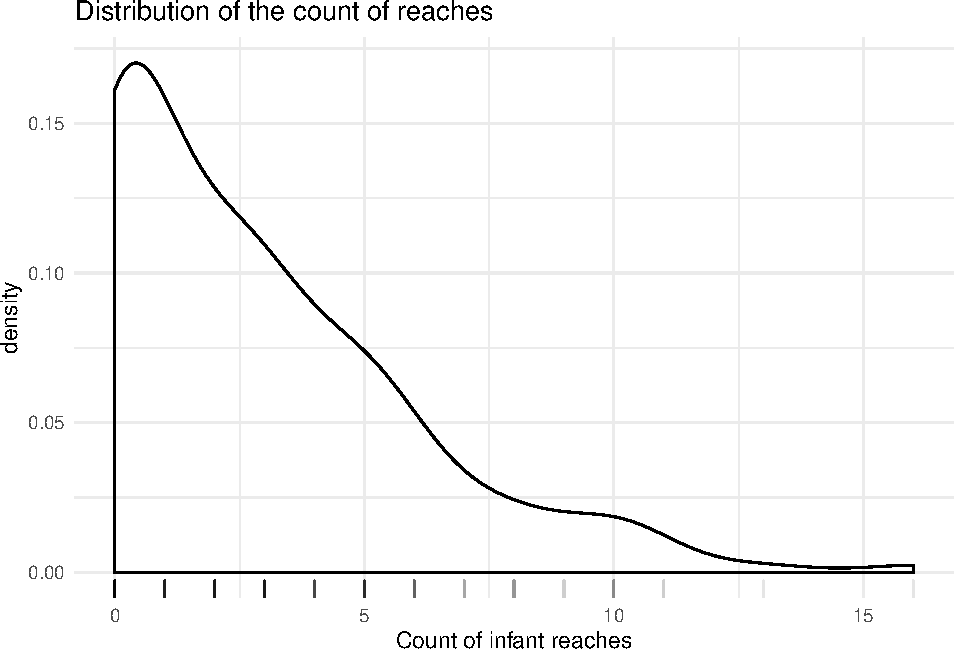
\includegraphics{supplement_files/figure-latex/reaches-1.pdf}

\begin{center}\rule{0.5\linewidth}{\linethickness}\end{center}

The following models test cultural group for infant reaches.

\begin{Shaded}
\begin{Highlighting}[]
\CommentTok{# Estimation of theta for the negbin() family}
\NormalTok{reach_nb <-}\StringTok{ }\KeywordTok{glm.nb}\NormalTok{(count }\OperatorTok{~}\StringTok{ }\NormalTok{months, }\DataTypeTok{data =}\NormalTok{ reach_tot)}
\NormalTok{theta <-}\StringTok{ }\KeywordTok{summary}\NormalTok{(reach_nb)[[}\StringTok{"theta"}\NormalTok{]]}

\NormalTok{reach_gam <-}\StringTok{ }\KeywordTok{gam}\NormalTok{(}
\NormalTok{  count }\OperatorTok{~}
\StringTok{    }\CommentTok{# parametric term}
\StringTok{    }\NormalTok{back_o }\OperatorTok{+}
\StringTok{    }\CommentTok{# reference smooth}
\StringTok{    }\KeywordTok{s}\NormalTok{(months, }\DataTypeTok{k =} \DecValTok{3}\NormalTok{) }\OperatorTok{+}
\StringTok{    }\CommentTok{# difference smoth}
\StringTok{    }\KeywordTok{s}\NormalTok{(months, }\DataTypeTok{k =} \DecValTok{3}\NormalTok{, }\DataTypeTok{by =}\NormalTok{ back_o) }\OperatorTok{+}
\StringTok{    }\CommentTok{# random smooths (random effect)}
\StringTok{    }\KeywordTok{s}\NormalTok{(months, dyad, }\DataTypeTok{k =} \DecValTok{2}\NormalTok{, }\DataTypeTok{bs =} \StringTok{"fs"}\NormalTok{, }\DataTypeTok{m =} \DecValTok{1}\NormalTok{),}
  \DataTypeTok{data =}\NormalTok{ reach_tot,}
  \DataTypeTok{method =} \StringTok{"ML"}\NormalTok{,}
  \DataTypeTok{family =} \KeywordTok{negbin}\NormalTok{(theta)}
\NormalTok{)}
\end{Highlighting}
\end{Shaded}

\begin{verbatim}
## Warning in gam.side(sm, X, tol = .Machine$double.eps^0.5): model has
## repeated 1-d smooths of same variable.
\end{verbatim}

\begin{Shaded}
\begin{Highlighting}[]
\KeywordTok{summary}\NormalTok{(reach_gam)}
\end{Highlighting}
\end{Shaded}

\begin{verbatim}
## 
## Family: Negative Binomial(0.986) 
## Link function: log 
## 
## Formula:
## count ~ back_o + s(months, k = 3) + s(months, k = 3, by = back_o) + 
##     s(months, dyad, k = 2, bs = "fs", m = 1)
## 
## Parametric coefficients:
##               Estimate Std. Error z value Pr(>|z|)    
## (Intercept)     0.6375     0.1920   3.321 0.000898 ***
## back_oBengali   0.5874     0.2601   2.258 0.023923 *  
## back_oChinese   0.2403     0.2651   0.906 0.364704    
## ---
## Signif. codes:  0 '***' 0.001 '**' 0.01 '*' 0.05 '.' 0.1 ' ' 1
## 
## Approximate significance of smooth terms:
##                            edf  Ref.df Chi.sq p-value  
## s(months)                1.156   1.287  1.181  0.2853  
## s(months):back_oBengali  1.000   1.000  0.437  0.5085  
## s(months):back_oChinese  1.000   1.000  0.125  0.7238  
## s(months,dyad)          14.522 112.000 20.065  0.0315 *
## ---
## Signif. codes:  0 '***' 0.001 '**' 0.01 '*' 0.05 '.' 0.1 ' ' 1
## 
## R-sq.(adj) =  0.165   Deviance explained = 21.4%
## -ML = 378.53  Scale est. = 1         n = 173
\end{verbatim}

\begin{Shaded}
\begin{Highlighting}[]
\NormalTok{reach_gam_null <-}\StringTok{ }\KeywordTok{gam}\NormalTok{(}
\NormalTok{  count }\OperatorTok{~}
\StringTok{    }\CommentTok{# back_o +}
\StringTok{    }\KeywordTok{s}\NormalTok{(months, }\DataTypeTok{k =} \DecValTok{3}\NormalTok{) }\OperatorTok{+}
\StringTok{    }\CommentTok{# s(months, k = 3, by = back_o) +}
\StringTok{    }\KeywordTok{s}\NormalTok{(months, dyad, }\DataTypeTok{k =} \DecValTok{2}\NormalTok{, }\DataTypeTok{bs =} \StringTok{"fs"}\NormalTok{, }\DataTypeTok{m =} \DecValTok{1}\NormalTok{),}
  \DataTypeTok{data =}\NormalTok{ reach_tot,}
  \DataTypeTok{method =} \StringTok{"ML"}\NormalTok{,}
  \DataTypeTok{family =} \KeywordTok{negbin}\NormalTok{(theta)}
\NormalTok{)}
\end{Highlighting}
\end{Shaded}

\begin{verbatim}
## Warning in gam.side(sm, X, tol = .Machine$double.eps^0.5): model has
## repeated 1-d smooths of same variable.
\end{verbatim}

\begin{Shaded}
\begin{Highlighting}[]
\KeywordTok{compareML}\NormalTok{(reach_gam_null, reach_gam)}
\end{Highlighting}
\end{Shaded}

\begin{verbatim}
## reach_gam_null: count ~ s(months, k = 3) + s(months, dyad, k = 2, bs = "fs", 
##     m = 1)
## 
## reach_gam: count ~ back_o + s(months, k = 3) + s(months, k = 3, by = back_o) + 
##     s(months, dyad, k = 2, bs = "fs", m = 1)
## 
## Chi-square test of ML scores
## -----
##            Model    Score Edf Difference    Df p.value Sig.
## 1 reach_gam_null 381.3235   5                              
## 2      reach_gam 378.5313  11      2.792 6.000   0.471     
## 
## AIC difference: -1.91, model reach_gam_null has lower AIC.
\end{verbatim}

\begin{verbatim}
## Warning in compareML(reach_gam_null, reach_gam): Only small difference in ML...
\end{verbatim}

\begin{Shaded}
\begin{Highlighting}[]
\KeywordTok{plot_smooths}\NormalTok{(reach_gam, months, }\DataTypeTok{facet_terms =}\NormalTok{ back_o, }\DataTypeTok{series_length =} \DecValTok{25}\NormalTok{, }\DataTypeTok{transform =}\NormalTok{ exp) }\OperatorTok{+}
\StringTok{  }\KeywordTok{labs}\NormalTok{(}\DataTypeTok{x =} \StringTok{"Months"}\NormalTok{, }\DataTypeTok{y =} \StringTok{"Count of reaches"}\NormalTok{, }\DataTypeTok{title =} \StringTok{"Predicted development of reaches by background"}\NormalTok{)}
\end{Highlighting}
\end{Shaded}

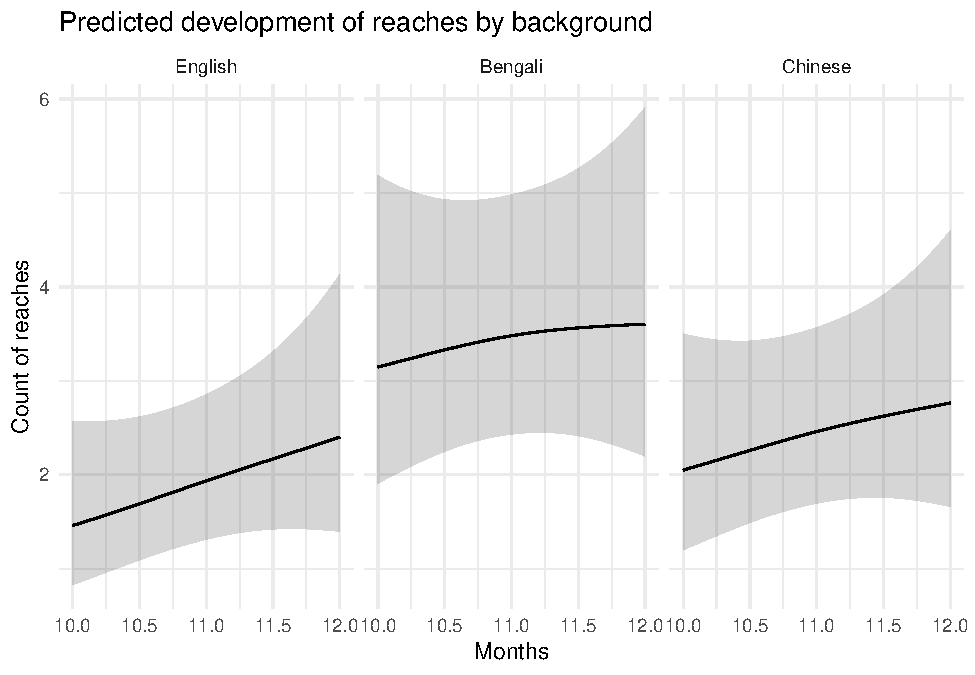
\includegraphics{supplement_files/figure-latex/reach-gam-plot-1.pdf}

\begin{center}\rule{0.5\linewidth}{\linethickness}\end{center}

The following models test the development of infant reaches.

\begin{Shaded}
\begin{Highlighting}[]
\NormalTok{reach_gam_}\DecValTok{2}\NormalTok{ <-}\StringTok{ }\KeywordTok{gam}\NormalTok{(}
\NormalTok{  count }\OperatorTok{~}
\StringTok{    }\KeywordTok{s}\NormalTok{(months, }\DataTypeTok{k =} \DecValTok{3}\NormalTok{) }\OperatorTok{+}
\StringTok{    }\KeywordTok{s}\NormalTok{(months, dyad, }\DataTypeTok{k =} \DecValTok{2}\NormalTok{, }\DataTypeTok{bs =} \StringTok{"fs"}\NormalTok{, }\DataTypeTok{m =} \DecValTok{1}\NormalTok{),}
  \DataTypeTok{data =}\NormalTok{ reach_tot,}
  \DataTypeTok{method =} \StringTok{"ML"}\NormalTok{,}
  \DataTypeTok{family =} \KeywordTok{negbin}\NormalTok{(theta)}
\NormalTok{)}
\end{Highlighting}
\end{Shaded}

\begin{verbatim}
## Warning in gam.side(sm, X, tol = .Machine$double.eps^0.5): model has
## repeated 1-d smooths of same variable.
\end{verbatim}

\begin{Shaded}
\begin{Highlighting}[]
\NormalTok{reach_gam_}\DecValTok{2}\NormalTok{_null <-}\StringTok{ }\KeywordTok{gam}\NormalTok{(}
\NormalTok{  count }\OperatorTok{~}
\StringTok{    }\CommentTok{# s(months, k = 3) +}
\StringTok{    }\KeywordTok{s}\NormalTok{(months, dyad, }\DataTypeTok{k =} \DecValTok{2}\NormalTok{, }\DataTypeTok{bs =} \StringTok{"fs"}\NormalTok{, }\DataTypeTok{m =} \DecValTok{1}\NormalTok{),}
  \DataTypeTok{data =}\NormalTok{ reach_tot,}
  \DataTypeTok{method =} \StringTok{"ML"}\NormalTok{,}
  \DataTypeTok{family =} \KeywordTok{negbin}\NormalTok{(theta)}
\NormalTok{)}
\KeywordTok{compareML}\NormalTok{(reach_gam_}\DecValTok{2}\NormalTok{_null, reach_gam_}\DecValTok{2}\NormalTok{)}
\end{Highlighting}
\end{Shaded}

\begin{verbatim}
## reach_gam_2_null: count ~ s(months, dyad, k = 2, bs = "fs", m = 1)
## 
## reach_gam_2: count ~ s(months, k = 3) + s(months, dyad, k = 2, bs = "fs", 
##     m = 1)
## 
## Chi-square test of ML scores
## -----
##              Model    Score Edf Difference    Df p.value Sig.
## 1 reach_gam_2_null 382.1529   3                              
## 2      reach_gam_2 381.3235   5      0.829 2.000   0.436     
## 
## AIC difference: -3.95, model reach_gam_2_null has lower AIC.
\end{verbatim}

\begin{verbatim}
## Warning in compareML(reach_gam_2_null, reach_gam_2): Only small difference in ML...
\end{verbatim}

\begin{Shaded}
\begin{Highlighting}[]
\KeywordTok{plot_smooths}\NormalTok{(reach_gam_}\DecValTok{2}\NormalTok{, months, }\DataTypeTok{series_length =} \DecValTok{25}\NormalTok{, }\DataTypeTok{transform =}\NormalTok{ exp) }\OperatorTok{+}
\StringTok{  }\KeywordTok{labs}\NormalTok{(}\DataTypeTok{x =} \StringTok{"Months"}\NormalTok{, }\DataTypeTok{y =} \StringTok{"Count of reaches"}\NormalTok{, }\DataTypeTok{title =} \StringTok{"Predicted development of reaches"}\NormalTok{)}
\end{Highlighting}
\end{Shaded}

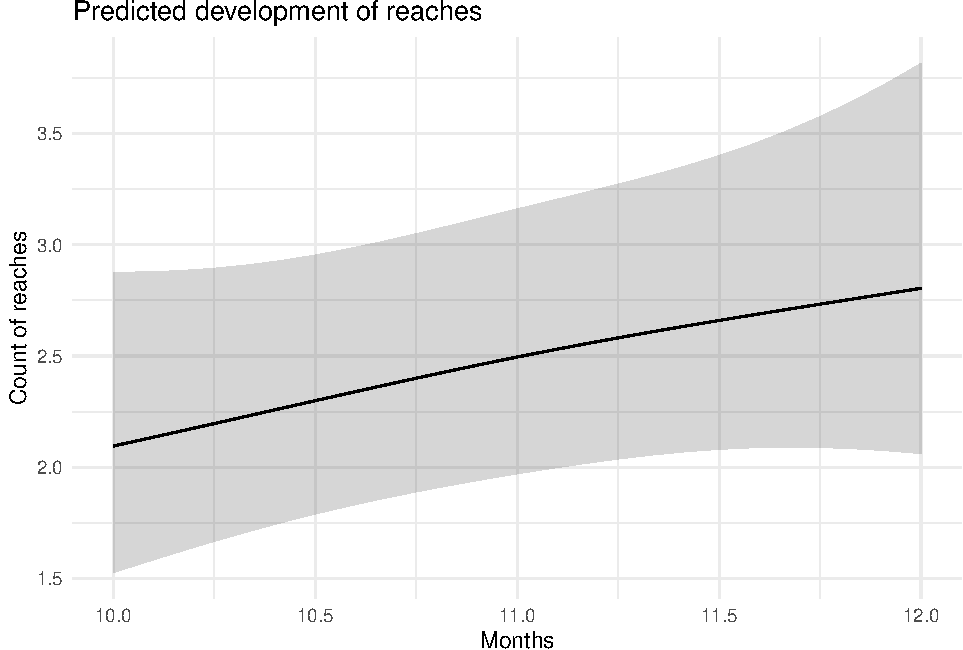
\includegraphics{supplement_files/figure-latex/reach-gam-2-plot-1.pdf}

\hypertarget{hgs-development}{%
\subsection{HGs development}\label{hgs-development}}

\begin{Shaded}
\begin{Highlighting}[]
\NormalTok{hg_tot }\OperatorTok
\StringTok{  }\KeywordTok{ggplot}\NormalTok{(}\KeywordTok{aes}\NormalTok{(count)) }\OperatorTok{+}\StringTok{ }\KeywordTok{geom_density}\NormalTok{() }\OperatorTok{+}\StringTok{ }\KeywordTok{geom_rug}\NormalTok{(}\DataTypeTok{alpha =} \FloatTok{0.1}\NormalTok{) }\OperatorTok{+}
\StringTok{  }\KeywordTok{labs}\NormalTok{(}
    \DataTypeTok{title =} \StringTok{"Distribution of the count of HoGs"}\NormalTok{,}
    \DataTypeTok{x =} \StringTok{"Count of infant HoGs"}
\NormalTok{  )}
\end{Highlighting}
\end{Shaded}

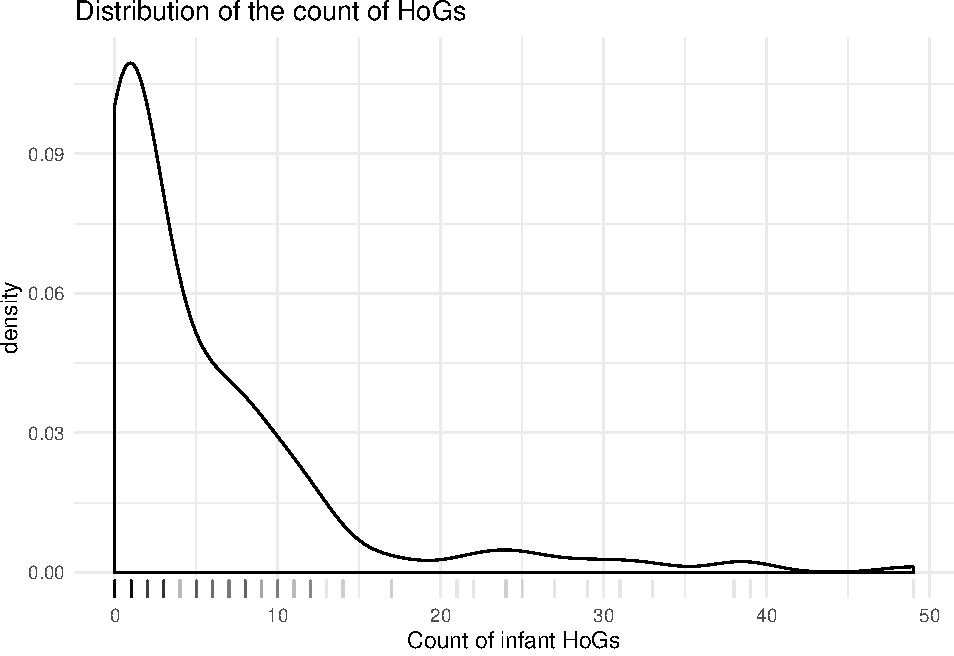
\includegraphics{supplement_files/figure-latex/hog-1.pdf}

\begin{center}\rule{0.5\linewidth}{\linethickness}\end{center}

The following models test cultural group differences for infant HoGs.

\begin{Shaded}
\begin{Highlighting}[]
\NormalTok{hg_nb <-}\StringTok{ }\KeywordTok{glm.nb}\NormalTok{(count }\OperatorTok{~}\StringTok{ }\NormalTok{months, }\DataTypeTok{data =}\NormalTok{ hg_tot)}
\NormalTok{theta_}\DecValTok{2}\NormalTok{ <-}\StringTok{ }\KeywordTok{summary}\NormalTok{(hg_nb)[[}\StringTok{"theta"}\NormalTok{]]}

\NormalTok{hg_gam <-}\StringTok{ }\KeywordTok{gam}\NormalTok{(}
\NormalTok{  count }\OperatorTok{~}
\StringTok{    }\NormalTok{back_o }\OperatorTok{+}
\StringTok{    }\KeywordTok{s}\NormalTok{(months, }\DataTypeTok{k =} \DecValTok{3}\NormalTok{) }\OperatorTok{+}
\StringTok{    }\KeywordTok{s}\NormalTok{(months, }\DataTypeTok{k =} \DecValTok{3}\NormalTok{, }\DataTypeTok{by =}\NormalTok{ back_o) }\OperatorTok{+}
\StringTok{    }\KeywordTok{s}\NormalTok{(months, dyad, }\DataTypeTok{k =} \DecValTok{2}\NormalTok{, }\DataTypeTok{bs =} \StringTok{"fs"}\NormalTok{, }\DataTypeTok{m =} \DecValTok{1}\NormalTok{),}
  \DataTypeTok{data =}\NormalTok{ hg_tot,}
  \DataTypeTok{method =} \StringTok{"ML"}\NormalTok{,}
  \DataTypeTok{family =} \KeywordTok{negbin}\NormalTok{(theta_}\DecValTok{2}\NormalTok{)}
\NormalTok{)}
\end{Highlighting}
\end{Shaded}

\begin{verbatim}
## Warning in gam.side(sm, X, tol = .Machine$double.eps^0.5): model has
## repeated 1-d smooths of same variable.
\end{verbatim}

\begin{Shaded}
\begin{Highlighting}[]
\KeywordTok{summary}\NormalTok{(hg_gam)}
\end{Highlighting}
\end{Shaded}

\begin{verbatim}
## 
## Family: Negative Binomial(0.643) 
## Link function: log 
## 
## Formula:
## count ~ back_o + s(months, k = 3) + s(months, k = 3, by = back_o) + 
##     s(months, dyad, k = 2, bs = "fs", m = 1)
## 
## Parametric coefficients:
##               Estimate Std. Error z value Pr(>|z|)   
## (Intercept)     0.7491     0.2316   3.234  0.00122 **
## back_oBengali   0.9117     0.3143   2.901  0.00372 **
## back_oChinese   0.7257     0.3163   2.295  0.02176 * 
## ---
## Signif. codes:  0 '***' 0.001 '**' 0.01 '*' 0.05 '.' 0.1 ' ' 1
## 
## Approximate significance of smooth terms:
##                           edf Ref.df Chi.sq p-value   
## s(months)                1.00      1  9.708 0.00184 **
## s(months):back_oBengali  1.00      1  0.025 0.87559   
## s(months):back_oChinese  1.00      1  0.426 0.51391   
## s(months,dyad)          17.71    112 26.332 0.01074 * 
## ---
## Signif. codes:  0 '***' 0.001 '**' 0.01 '*' 0.05 '.' 0.1 ' ' 1
## 
## R-sq.(adj) =  0.335   Deviance explained = 38.5%
## -ML = 451.06  Scale est. = 1         n = 173
\end{verbatim}

\begin{Shaded}
\begin{Highlighting}[]
\NormalTok{hg_gam_null <-}\StringTok{ }\KeywordTok{gam}\NormalTok{(}
\NormalTok{  count }\OperatorTok{~}
\StringTok{    }\CommentTok{# back_o +}
\StringTok{    }\KeywordTok{s}\NormalTok{(months, }\DataTypeTok{k =} \DecValTok{3}\NormalTok{) }\OperatorTok{+}
\StringTok{    }\CommentTok{# s(months, k = 3, by = back_o) +}
\StringTok{    }\KeywordTok{s}\NormalTok{(months, dyad, }\DataTypeTok{k =} \DecValTok{2}\NormalTok{, }\DataTypeTok{bs =} \StringTok{"fs"}\NormalTok{, }\DataTypeTok{m =} \DecValTok{1}\NormalTok{),}
  \DataTypeTok{data =}\NormalTok{ hg_tot,}
  \DataTypeTok{method =} \StringTok{"ML"}\NormalTok{,}
  \DataTypeTok{family =} \KeywordTok{negbin}\NormalTok{(theta_}\DecValTok{2}\NormalTok{)}
\NormalTok{)}
\end{Highlighting}
\end{Shaded}

\begin{verbatim}
## Warning in gam.side(sm, X, tol = .Machine$double.eps^0.5): model has
## repeated 1-d smooths of same variable.
\end{verbatim}

\begin{Shaded}
\begin{Highlighting}[]
\KeywordTok{compareML}\NormalTok{(hg_gam_null, hg_gam)}
\end{Highlighting}
\end{Shaded}

\begin{verbatim}
## hg_gam_null: count ~ s(months, k = 3) + s(months, dyad, k = 2, bs = "fs", 
##     m = 1)
## 
## hg_gam: count ~ back_o + s(months, k = 3) + s(months, k = 3, by = back_o) + 
##     s(months, dyad, k = 2, bs = "fs", m = 1)
## 
## Chi-square test of ML scores
## -----
##         Model    Score Edf Difference    Df p.value Sig.
## 1 hg_gam_null 455.3692   5                              
## 2      hg_gam 451.0596  11      4.310 6.000   0.196     
## 
## AIC difference: -2.20, model hg_gam_null has lower AIC.
\end{verbatim}

\begin{verbatim}
## Warning in compareML(hg_gam_null, hg_gam): Only small difference in ML...
\end{verbatim}

\begin{Shaded}
\begin{Highlighting}[]
\KeywordTok{plot_smooths}\NormalTok{(hg_gam, months, }\DataTypeTok{facet_terms =}\NormalTok{ back_o, }\DataTypeTok{series_length =} \DecValTok{25}\NormalTok{, }\DataTypeTok{transform =}\NormalTok{ exp) }\OperatorTok{+}
\StringTok{  }\KeywordTok{labs}\NormalTok{(}\DataTypeTok{x =} \StringTok{"Months"}\NormalTok{, }\DataTypeTok{y =} \StringTok{"Count of HoGs"}\NormalTok{, }\DataTypeTok{title =} \StringTok{"Predicted development of HoGs by background"}\NormalTok{)}
\end{Highlighting}
\end{Shaded}

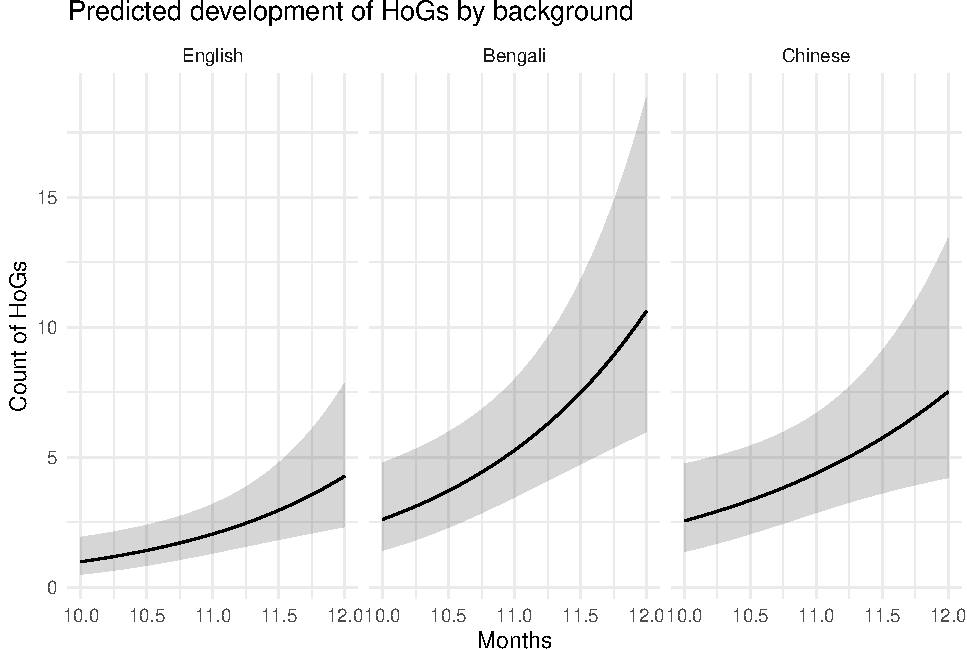
\includegraphics{supplement_files/figure-latex/hg-gam-plot-1.pdf}

\begin{center}\rule{0.5\linewidth}{\linethickness}\end{center}

The following models test development of infant HoGs.

\begin{Shaded}
\begin{Highlighting}[]
\NormalTok{hg_gam_}\DecValTok{2}\NormalTok{ <-}\StringTok{ }\KeywordTok{gam}\NormalTok{(}
\NormalTok{  count }\OperatorTok{~}
\StringTok{    }\KeywordTok{s}\NormalTok{(months, }\DataTypeTok{k =} \DecValTok{3}\NormalTok{) }\OperatorTok{+}
\StringTok{    }\KeywordTok{s}\NormalTok{(months, dyad, }\DataTypeTok{k =} \DecValTok{2}\NormalTok{, }\DataTypeTok{bs =} \StringTok{"fs"}\NormalTok{, }\DataTypeTok{m =} \DecValTok{1}\NormalTok{),}
  \DataTypeTok{data =}\NormalTok{ hg_tot,}
  \DataTypeTok{method =} \StringTok{"ML"}\NormalTok{,}
  \DataTypeTok{family =} \KeywordTok{negbin}\NormalTok{(theta_}\DecValTok{2}\NormalTok{)}
\NormalTok{)}
\end{Highlighting}
\end{Shaded}

\begin{verbatim}
## Warning in gam.side(sm, X, tol = .Machine$double.eps^0.5): model has
## repeated 1-d smooths of same variable.
\end{verbatim}

\begin{Shaded}
\begin{Highlighting}[]
\NormalTok{hg_gam_}\DecValTok{2}\NormalTok{_null <-}\StringTok{ }\KeywordTok{gam}\NormalTok{(}
\NormalTok{  count }\OperatorTok{~}
\StringTok{    }\CommentTok{# s(months, k = 3) +}
\StringTok{    }\KeywordTok{s}\NormalTok{(months, dyad, }\DataTypeTok{k =} \DecValTok{2}\NormalTok{, }\DataTypeTok{bs =} \StringTok{"fs"}\NormalTok{, }\DataTypeTok{m =} \DecValTok{1}\NormalTok{),}
  \DataTypeTok{data =}\NormalTok{ hg_tot,}
  \DataTypeTok{method =} \StringTok{"ML"}\NormalTok{,}
  \DataTypeTok{family =} \KeywordTok{negbin}\NormalTok{(theta_}\DecValTok{2}\NormalTok{)}
\NormalTok{)}
\KeywordTok{compareML}\NormalTok{(hg_gam_}\DecValTok{2}\NormalTok{_null, hg_gam_}\DecValTok{2}\NormalTok{)}
\end{Highlighting}
\end{Shaded}

\begin{verbatim}
## hg_gam_2_null: count ~ s(months, dyad, k = 2, bs = "fs", m = 1)
## 
## hg_gam_2: count ~ s(months, k = 3) + s(months, dyad, k = 2, bs = "fs", 
##     m = 1)
## 
## Chi-square test of ML scores
## -----
##           Model    Score Edf Difference    Df   p.value Sig.
## 1 hg_gam_2_null 467.6971   3                                
## 2      hg_gam_2 455.3692   5     12.328 2.000 4.427e-06  ***
## 
## AIC difference: 29.27, model hg_gam_2 has lower AIC.
\end{verbatim}

\begin{Shaded}
\begin{Highlighting}[]
\KeywordTok{plot_smooths}\NormalTok{(hg_gam_}\DecValTok{2}\NormalTok{, months, }\DataTypeTok{series_length =} \DecValTok{25}\NormalTok{, }\DataTypeTok{transform =}\NormalTok{ exp) }\OperatorTok{+}
\StringTok{  }\KeywordTok{labs}\NormalTok{(}\DataTypeTok{x =} \StringTok{"Months"}\NormalTok{, }\DataTypeTok{y =} \StringTok{"Count of HoGs"}\NormalTok{, }\DataTypeTok{title =} \StringTok{"Predicted development of HoGs"}\NormalTok{)}
\end{Highlighting}
\end{Shaded}

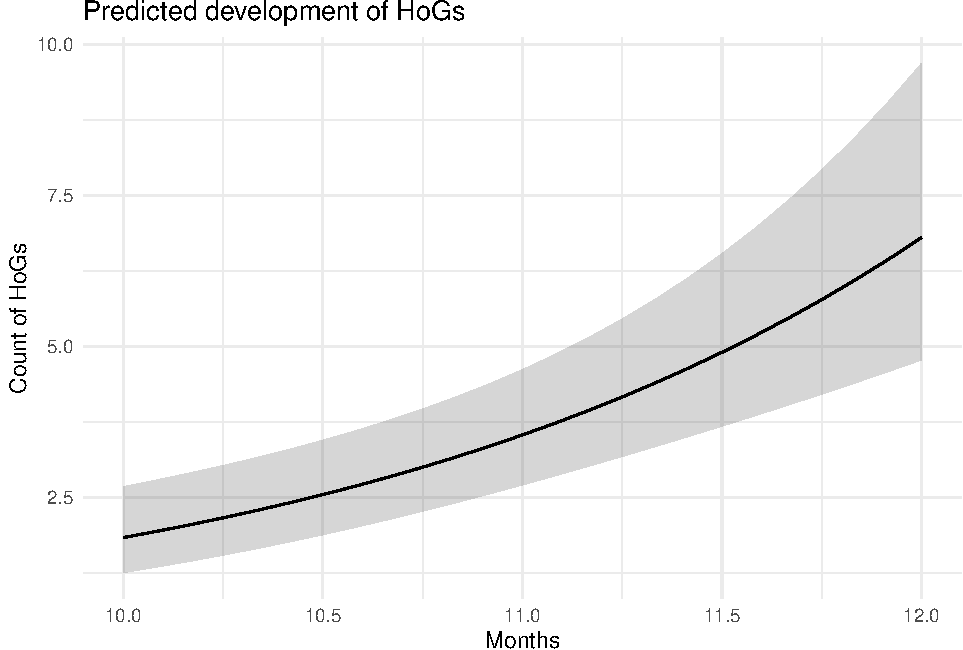
\includegraphics{supplement_files/figure-latex/hg-gam-2-plot-1.pdf}

\hypertarget{points-development}{%
\subsection{Points development}\label{points-development}}

\begin{Shaded}
\begin{Highlighting}[]
\NormalTok{point_tot }\OperatorTok
\StringTok{  }\KeywordTok{ggplot}\NormalTok{(}\KeywordTok{aes}\NormalTok{(count)) }\OperatorTok{+}\StringTok{ }\KeywordTok{geom_density}\NormalTok{() }\OperatorTok{+}\StringTok{ }\KeywordTok{geom_rug}\NormalTok{(}\DataTypeTok{alpha =} \FloatTok{0.1}\NormalTok{) }\OperatorTok{+}
\StringTok{  }\KeywordTok{labs}\NormalTok{(}
    \DataTypeTok{title =} \StringTok{"Distribution of the count of points"}\NormalTok{,}
    \DataTypeTok{x =} \StringTok{"Count of infant points"}
\NormalTok{  )}
\end{Highlighting}
\end{Shaded}

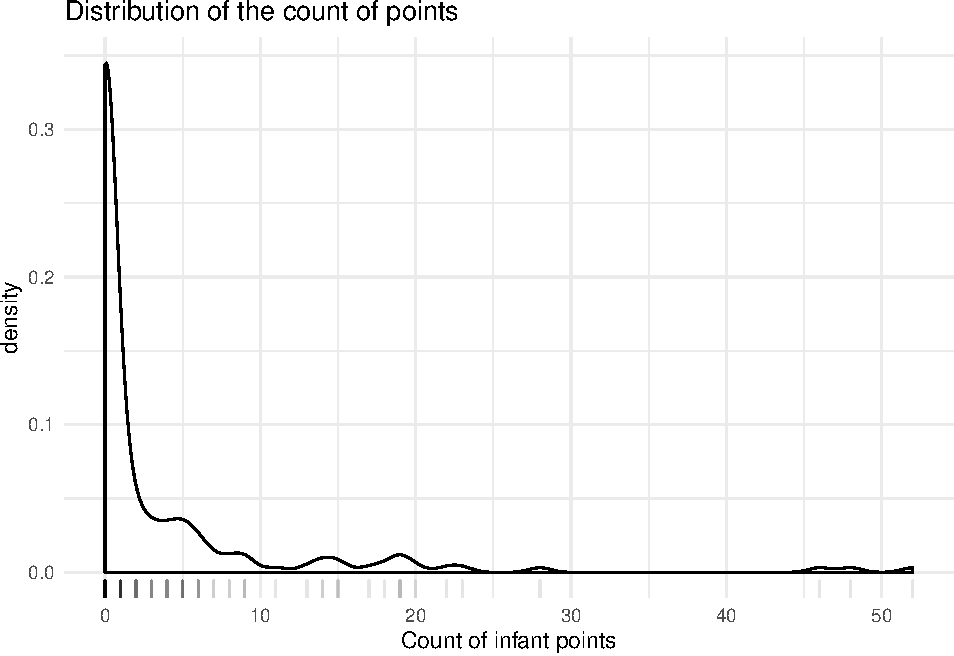
\includegraphics{supplement_files/figure-latex/points-1.pdf}

\begin{center}\rule{0.5\linewidth}{\linethickness}\end{center}

The following models test cultural group differences in infant pointing.

\begin{Shaded}
\begin{Highlighting}[]
\NormalTok{point_nb <-}\StringTok{ }\KeywordTok{glm.nb}\NormalTok{(count }\OperatorTok{~}\StringTok{ }\NormalTok{months, }\DataTypeTok{data =}\NormalTok{ point_tot)}
\NormalTok{theta_}\DecValTok{3}\NormalTok{ <-}\StringTok{ }\KeywordTok{summary}\NormalTok{(point_nb)[[}\StringTok{"theta"}\NormalTok{]]}

\NormalTok{point_gam <-}\StringTok{ }\KeywordTok{gam}\NormalTok{(}
\NormalTok{  count }\OperatorTok{~}
\StringTok{    }\NormalTok{back_o }\OperatorTok{+}
\StringTok{    }\KeywordTok{s}\NormalTok{(months, }\DataTypeTok{k =} \DecValTok{3}\NormalTok{) }\OperatorTok{+}
\StringTok{    }\KeywordTok{s}\NormalTok{(months, }\DataTypeTok{k =} \DecValTok{3}\NormalTok{, }\DataTypeTok{by =}\NormalTok{ back_o) }\OperatorTok{+}
\StringTok{    }\KeywordTok{s}\NormalTok{(months, dyad, }\DataTypeTok{k =} \DecValTok{2}\NormalTok{, }\DataTypeTok{bs =} \StringTok{"fs"}\NormalTok{, }\DataTypeTok{m =} \DecValTok{1}\NormalTok{),}
  \DataTypeTok{data =}\NormalTok{ point_tot,}
  \DataTypeTok{method =} \StringTok{"ML"}\NormalTok{,}
  \DataTypeTok{family =} \KeywordTok{negbin}\NormalTok{(theta_}\DecValTok{3}\NormalTok{)}
\NormalTok{)}
\end{Highlighting}
\end{Shaded}

\begin{verbatim}
## Warning in gam.side(sm, X, tol = .Machine$double.eps^0.5): model has
## repeated 1-d smooths of same variable.
\end{verbatim}

\begin{Shaded}
\begin{Highlighting}[]
\KeywordTok{summary}\NormalTok{(point_gam)}
\end{Highlighting}
\end{Shaded}

\begin{verbatim}
## 
## Family: Negative Binomial(0.195) 
## Link function: log 
## 
## Formula:
## count ~ back_o + s(months, k = 3) + s(months, k = 3, by = back_o) + 
##     s(months, dyad, k = 2, bs = "fs", m = 1)
## 
## Parametric coefficients:
##               Estimate Std. Error z value Pr(>|z|)  
## (Intercept)     0.6919     0.3953   1.750   0.0801 .
## back_oBengali  -0.4994     0.5588  -0.894   0.3715  
## back_oChinese  -0.5735     0.5675  -1.011   0.3122  
## ---
## Signif. codes:  0 '***' 0.001 '**' 0.01 '*' 0.05 '.' 0.1 ' ' 1
## 
## Approximate significance of smooth terms:
##                            edf  Ref.df Chi.sq p-value  
## s(months)                1.000   1.000  1.068  0.3014  
## s(months):back_oBengali  1.538   1.786  0.726  0.5737  
## s(months):back_oChinese  1.000   1.000  2.118  0.1456  
## s(months,dyad)          18.368 112.000 25.998  0.0225 *
## ---
## Signif. codes:  0 '***' 0.001 '**' 0.01 '*' 0.05 '.' 0.1 ' ' 1
## 
## R-sq.(adj) =  0.332   Deviance explained =   41%
## -ML = 326.24  Scale est. = 1         n = 173
\end{verbatim}

\begin{Shaded}
\begin{Highlighting}[]
\NormalTok{point_gam_null <-}\StringTok{ }\KeywordTok{gam}\NormalTok{(}
\NormalTok{  count }\OperatorTok{~}
\StringTok{    }\CommentTok{# back_o +}
\StringTok{    }\KeywordTok{s}\NormalTok{(months, }\DataTypeTok{k =} \DecValTok{3}\NormalTok{) }\OperatorTok{+}
\StringTok{    }\CommentTok{# s(months, k = 3, by = back_o) +}
\StringTok{    }\KeywordTok{s}\NormalTok{(months, dyad, }\DataTypeTok{k =} \DecValTok{2}\NormalTok{, }\DataTypeTok{bs =} \StringTok{"fs"}\NormalTok{, }\DataTypeTok{m =} \DecValTok{1}\NormalTok{),}
  \DataTypeTok{data =}\NormalTok{ point_tot,}
  \DataTypeTok{method =} \StringTok{"ML"}\NormalTok{,}
  \DataTypeTok{family =} \KeywordTok{negbin}\NormalTok{(theta_}\DecValTok{3}\NormalTok{)}
\NormalTok{)}
\end{Highlighting}
\end{Shaded}

\begin{verbatim}
## Warning in gam.side(sm, X, tol = .Machine$double.eps^0.5): model has
## repeated 1-d smooths of same variable.
\end{verbatim}

\begin{Shaded}
\begin{Highlighting}[]
\KeywordTok{compareML}\NormalTok{(point_gam_null, point_gam)}
\end{Highlighting}
\end{Shaded}

\begin{verbatim}
## point_gam_null: count ~ s(months, k = 3) + s(months, dyad, k = 2, bs = "fs", 
##     m = 1)
## 
## point_gam: count ~ back_o + s(months, k = 3) + s(months, k = 3, by = back_o) + 
##     s(months, dyad, k = 2, bs = "fs", m = 1)
## 
## Chi-square test of ML scores
## -----
##            Model    Score Edf Difference    Df p.value Sig.
## 1 point_gam_null 327.9371   5                              
## 2      point_gam 326.2371  11      1.700 6.000   0.757     
## 
## AIC difference: -7.40, model point_gam_null has lower AIC.
\end{verbatim}

\begin{verbatim}
## Warning in compareML(point_gam_null, point_gam): Only small difference in ML...
\end{verbatim}

\begin{Shaded}
\begin{Highlighting}[]
\KeywordTok{plot_smooths}\NormalTok{(point_gam, months, }\DataTypeTok{facet_terms =}\NormalTok{ back_o, }\DataTypeTok{series_length =} \DecValTok{25}\NormalTok{, }\DataTypeTok{transform =}\NormalTok{ exp) }\OperatorTok{+}
\StringTok{  }\KeywordTok{labs}\NormalTok{(}\DataTypeTok{x =} \StringTok{"Months"}\NormalTok{, }\DataTypeTok{y =} \StringTok{"Count of points"}\NormalTok{, }\DataTypeTok{title =} \StringTok{"Predicted development of points by background"}\NormalTok{)}
\end{Highlighting}
\end{Shaded}

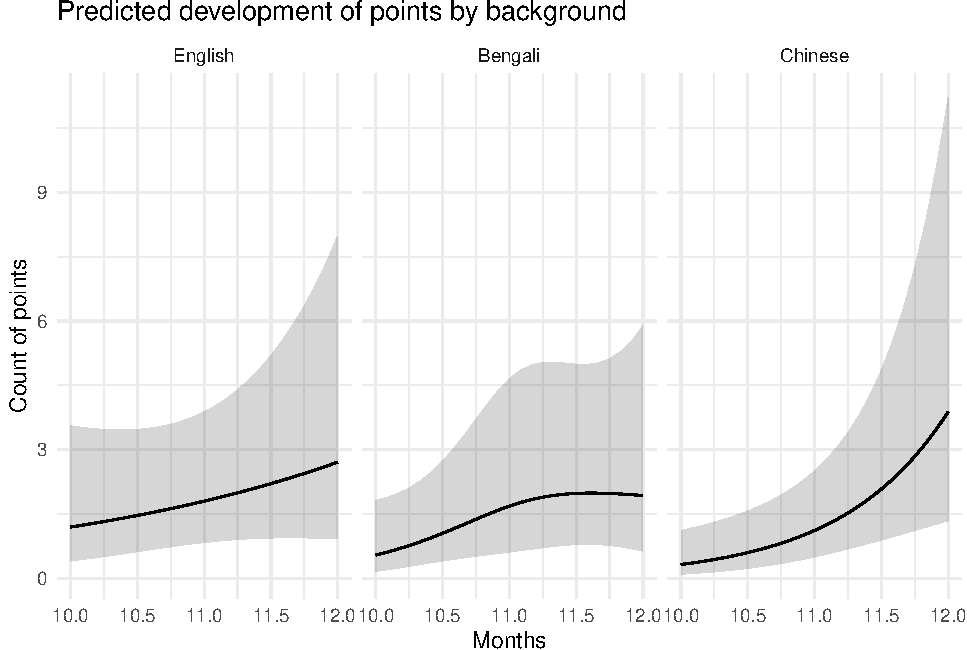
\includegraphics{supplement_files/figure-latex/point-gam-plot-1.pdf}

\begin{center}\rule{0.5\linewidth}{\linethickness}\end{center}

The following models test development of infant pointing.

\begin{Shaded}
\begin{Highlighting}[]
\NormalTok{point_gam_}\DecValTok{2}\NormalTok{ <-}\StringTok{ }\KeywordTok{gam}\NormalTok{(}
\NormalTok{  count }\OperatorTok{~}
\StringTok{    }\KeywordTok{s}\NormalTok{(months, }\DataTypeTok{k =} \DecValTok{3}\NormalTok{) }\OperatorTok{+}
\StringTok{    }\KeywordTok{s}\NormalTok{(months, dyad, }\DataTypeTok{k =} \DecValTok{2}\NormalTok{, }\DataTypeTok{bs =} \StringTok{"fs"}\NormalTok{, }\DataTypeTok{m =} \DecValTok{1}\NormalTok{),}
  \DataTypeTok{data =}\NormalTok{ point_tot,}
  \DataTypeTok{method =} \StringTok{"ML"}\NormalTok{,}
  \DataTypeTok{family =} \KeywordTok{negbin}\NormalTok{(theta_}\DecValTok{3}\NormalTok{)}
\NormalTok{)}
\end{Highlighting}
\end{Shaded}

\begin{verbatim}
## Warning in gam.side(sm, X, tol = .Machine$double.eps^0.5): model has
## repeated 1-d smooths of same variable.
\end{verbatim}

\begin{Shaded}
\begin{Highlighting}[]
\NormalTok{point_gam_}\DecValTok{2}\NormalTok{_null <-}\StringTok{ }\KeywordTok{gam}\NormalTok{(}
\NormalTok{  count }\OperatorTok{~}
\StringTok{    }\CommentTok{# s(months, k = 3) +}
\StringTok{    }\KeywordTok{s}\NormalTok{(months, dyad, }\DataTypeTok{k =} \DecValTok{2}\NormalTok{, }\DataTypeTok{bs =} \StringTok{"fs"}\NormalTok{, }\DataTypeTok{m =} \DecValTok{1}\NormalTok{),}
  \DataTypeTok{data =}\NormalTok{ point_tot,}
  \DataTypeTok{method =} \StringTok{"ML"}\NormalTok{,}
  \DataTypeTok{family =} \KeywordTok{negbin}\NormalTok{(theta_}\DecValTok{3}\NormalTok{)}
\NormalTok{)}
\KeywordTok{compareML}\NormalTok{(point_gam_}\DecValTok{2}\NormalTok{_null, point_gam_}\DecValTok{2}\NormalTok{)}
\end{Highlighting}
\end{Shaded}

\begin{verbatim}
## point_gam_2_null: count ~ s(months, dyad, k = 2, bs = "fs", m = 1)
## 
## point_gam_2: count ~ s(months, k = 3) + s(months, dyad, k = 2, bs = "fs", 
##     m = 1)
## 
## Chi-square test of ML scores
## -----
##              Model    Score Edf Difference    Df p.value Sig.
## 1 point_gam_2_null 332.5523   3                              
## 2      point_gam_2 327.9371   5      4.615 2.000   0.010  ** 
## 
## AIC difference: 10.13, model point_gam_2 has lower AIC.
\end{verbatim}

\begin{verbatim}
## Warning in compareML(point_gam_2_null, point_gam_2): Only small difference in ML...
\end{verbatim}

\begin{Shaded}
\begin{Highlighting}[]
\KeywordTok{plot_smooths}\NormalTok{(point_gam_}\DecValTok{2}\NormalTok{, months, }\DataTypeTok{series_length =} \DecValTok{25}\NormalTok{, }\DataTypeTok{transform =}\NormalTok{ exp) }\OperatorTok{+}
\StringTok{  }\KeywordTok{labs}\NormalTok{(}\DataTypeTok{x =} \StringTok{"Months"}\NormalTok{, }\DataTypeTok{y =} \StringTok{"Count of points"}\NormalTok{, }\DataTypeTok{title =} \StringTok{"Predicted development of points"}\NormalTok{)}
\end{Highlighting}
\end{Shaded}

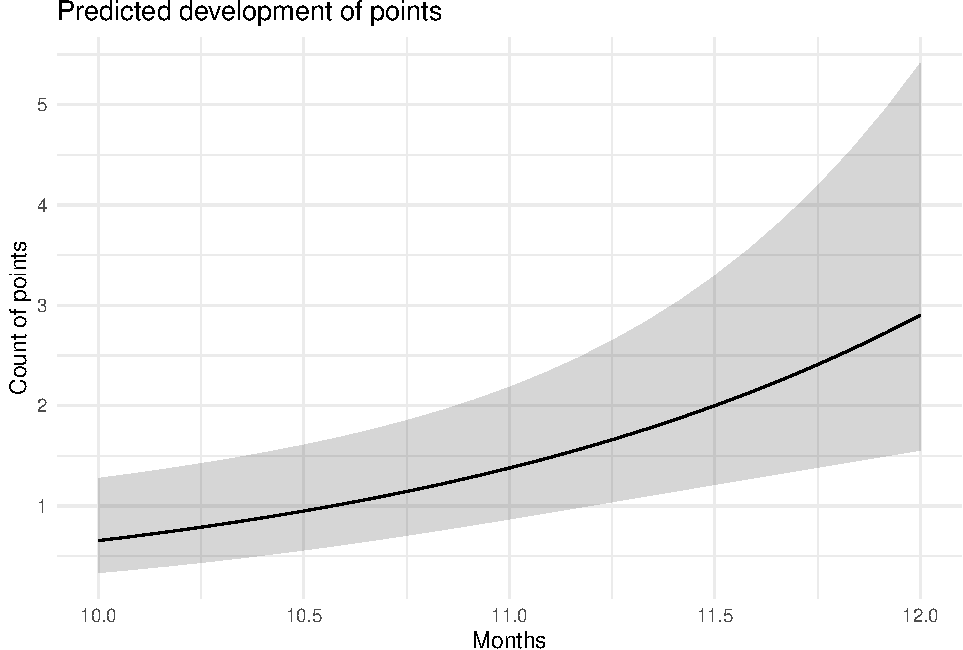
\includegraphics{supplement_files/figure-latex/point-gam-2-plot-1.pdf}

\newpage

\hypertarget{analysis-1b.-frequency-of-maternal-utterances-and-contingent-talk-to-infants-aged-10-12-months.}{%
\section{Analysis 1b. Frequency of maternal utterances and contingent
talk to infants aged 10-12
months.}\label{analysis-1b.-frequency-of-maternal-utterances-and-contingent-talk-to-infants-aged-10-12-months.}}

For maternal utterances we used a normal distribution, since the
distribution of the data was almost normal. For maternal contingent
talks instead we used again the negative binomial distribution for the
same reasons as above.

\hypertarget{maternal-utterances-development}{%
\subsection{Maternal utterances
development}\label{maternal-utterances-development}}

\begin{Shaded}
\begin{Highlighting}[]
\NormalTok{utterances_tot }\OperatorTok
\StringTok{  }\KeywordTok{ggplot}\NormalTok{(}\KeywordTok{aes}\NormalTok{(utterances)) }\OperatorTok{+}\StringTok{ }\KeywordTok{geom_density}\NormalTok{() }\OperatorTok{+}\StringTok{ }\KeywordTok{geom_rug}\NormalTok{(}\DataTypeTok{alpha =} \FloatTok{0.1}\NormalTok{) }\OperatorTok{+}
\StringTok{  }\KeywordTok{labs}\NormalTok{(}
    \DataTypeTok{title =} \StringTok{"Distribution of the count of utterances"}\NormalTok{,}
    \DataTypeTok{x =} \StringTok{"Count of maternal utterances"}
\NormalTok{  )}
\end{Highlighting}
\end{Shaded}

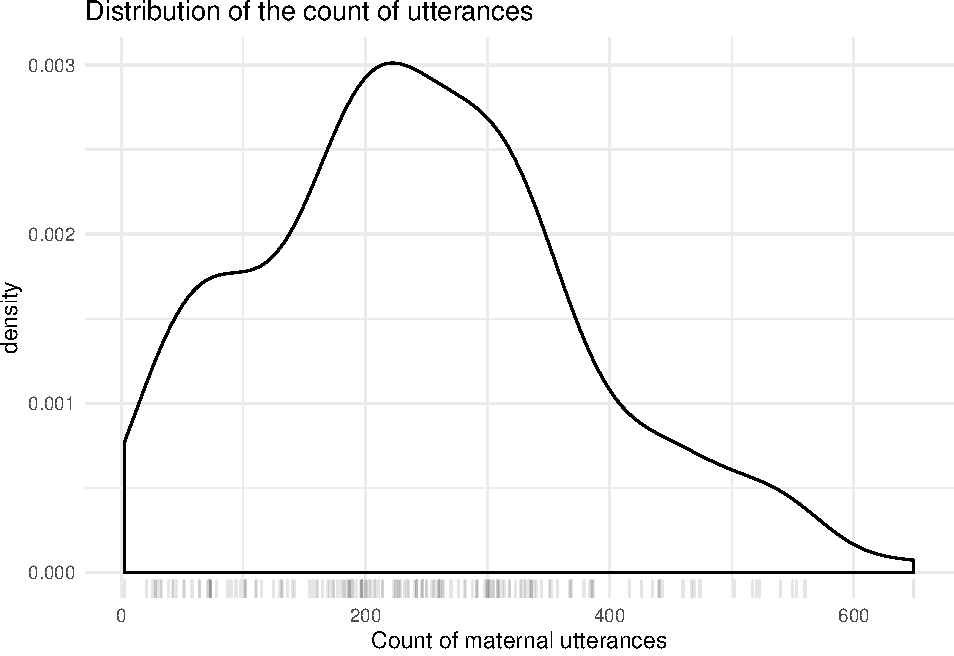
\includegraphics{supplement_files/figure-latex/utterances-1.pdf}

\begin{center}\rule{0.5\linewidth}{\linethickness}\end{center}

The following models test cultural group.

\begin{Shaded}
\begin{Highlighting}[]
\NormalTok{utter_gam <-}\StringTok{ }\KeywordTok{gam}\NormalTok{(}
\NormalTok{  utterances }\OperatorTok{~}
\StringTok{    }\NormalTok{back_o }\OperatorTok{+}
\StringTok{    }\KeywordTok{s}\NormalTok{(months, }\DataTypeTok{k =} \DecValTok{3}\NormalTok{) }\OperatorTok{+}
\StringTok{    }\KeywordTok{s}\NormalTok{(months, }\DataTypeTok{k =} \DecValTok{3}\NormalTok{, }\DataTypeTok{by =}\NormalTok{ back_o) }\OperatorTok{+}
\StringTok{    }\KeywordTok{s}\NormalTok{(months, dyad, }\DataTypeTok{k =} \DecValTok{2}\NormalTok{, }\DataTypeTok{bs =} \StringTok{"fs"}\NormalTok{, }\DataTypeTok{m =} \DecValTok{1}\NormalTok{),}
  \DataTypeTok{data =}\NormalTok{ utterances_tot,}
  \DataTypeTok{method =} \StringTok{"ML"}
\NormalTok{)}
\end{Highlighting}
\end{Shaded}

\begin{verbatim}
## Warning in gam.side(sm, X, tol = .Machine$double.eps^0.5): model has
## repeated 1-d smooths of same variable.
\end{verbatim}

\begin{Shaded}
\begin{Highlighting}[]
\KeywordTok{summary}\NormalTok{(utter_gam)}
\end{Highlighting}
\end{Shaded}

\begin{verbatim}
## 
## Family: gaussian 
## Link function: identity 
## 
## Formula:
## utterances ~ back_o + s(months, k = 3) + s(months, k = 3, by = back_o) + 
##     s(months, dyad, k = 2, bs = "fs", m = 1)
## 
## Parametric coefficients:
##               Estimate Std. Error t value Pr(>|t|)    
## (Intercept)     284.44      27.10  10.494   <2e-16 ***
## back_oBengali   -65.59      37.82  -1.734   0.0865 .  
## back_oChinese   -37.80      37.74  -1.002   0.3193    
## ---
## Signif. codes:  0 '***' 0.001 '**' 0.01 '*' 0.05 '.' 0.1 ' ' 1
## 
## Approximate significance of smooth terms:
##                            edf  Ref.df     F p-value    
## s(months)                1.693   1.880 0.966   0.333    
## s(months):back_oBengali  1.001   1.001 1.065   0.305    
## s(months):back_oChinese  1.334   1.533 1.924   0.107    
## s(months,dyad)          73.930 111.000 7.087  <2e-16 ***
## ---
## Signif. codes:  0 '***' 0.001 '**' 0.01 '*' 0.05 '.' 0.1 ' ' 1
## 
## R-sq.(adj) =  0.837   Deviance explained = 91.6%
## -ML = 991.97  Scale est. = 2827.4    n = 167
\end{verbatim}

\begin{Shaded}
\begin{Highlighting}[]
\NormalTok{utter_gam_null <-}\StringTok{ }\KeywordTok{gam}\NormalTok{(}
\NormalTok{  utterances }\OperatorTok{~}
\StringTok{    }\CommentTok{# back_o +}
\StringTok{    }\KeywordTok{s}\NormalTok{(months, }\DataTypeTok{k =} \DecValTok{3}\NormalTok{) }\OperatorTok{+}
\StringTok{    }\CommentTok{# s(months, k = 3, by = back_o) +}
\StringTok{    }\KeywordTok{s}\NormalTok{(months, dyad, }\DataTypeTok{k =} \DecValTok{2}\NormalTok{, }\DataTypeTok{bs =} \StringTok{"fs"}\NormalTok{, }\DataTypeTok{m =} \DecValTok{1}\NormalTok{),}
  \DataTypeTok{data =}\NormalTok{ utterances_tot,}
  \DataTypeTok{method =} \StringTok{"ML"}
\NormalTok{)}
\end{Highlighting}
\end{Shaded}

\begin{verbatim}
## Warning in gam.side(sm, X, tol = .Machine$double.eps^0.5): model has
## repeated 1-d smooths of same variable.
\end{verbatim}

\begin{Shaded}
\begin{Highlighting}[]
\KeywordTok{compareML}\NormalTok{(utter_gam_null, utter_gam)}
\end{Highlighting}
\end{Shaded}

\begin{verbatim}
## utter_gam_null: utterances ~ s(months, k = 3) + s(months, dyad, k = 2, bs = "fs", 
##     m = 1)
## 
## utter_gam: utterances ~ back_o + s(months, k = 3) + s(months, k = 3, by = back_o) + 
##     s(months, dyad, k = 2, bs = "fs", m = 1)
## 
## Chi-square test of ML scores
## -----
##            Model    Score Edf Difference    Df p.value Sig.
## 1 utter_gam_null 995.3291   5                              
## 2      utter_gam 991.9724  11      3.357 6.000   0.348     
## 
## AIC difference: -3.68, model utter_gam_null has lower AIC.
\end{verbatim}

\begin{verbatim}
## Warning in compareML(utter_gam_null, utter_gam): Only small difference in ML...
\end{verbatim}

\begin{Shaded}
\begin{Highlighting}[]
\KeywordTok{plot_smooths}\NormalTok{(utter_gam, months, }\DataTypeTok{facet_terms =}\NormalTok{ back_o, }\DataTypeTok{series_length =} \DecValTok{10}\NormalTok{) }\OperatorTok{+}
\StringTok{  }\KeywordTok{labs}\NormalTok{(}\DataTypeTok{x =} \StringTok{"Months"}\NormalTok{, }\DataTypeTok{y =} \StringTok{"Count of utterances"}\NormalTok{, }\DataTypeTok{title =} \StringTok{"Predicted development of utterances by background"}\NormalTok{)}
\end{Highlighting}
\end{Shaded}

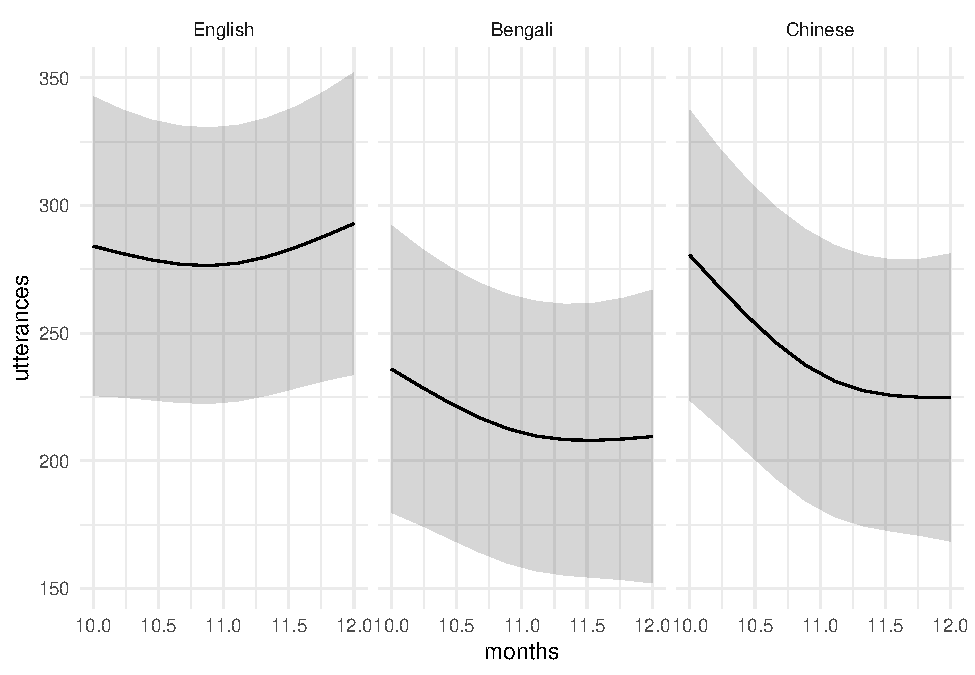
\includegraphics{supplement_files/figure-latex/utter-gam-plot-1.pdf}

\begin{center}\rule{0.5\linewidth}{\linethickness}\end{center}

The following models test time sample.

\begin{Shaded}
\begin{Highlighting}[]
\NormalTok{utter_gam_}\DecValTok{2}\NormalTok{ <-}\StringTok{ }\KeywordTok{gam}\NormalTok{(}
\NormalTok{  utterances }\OperatorTok{~}
\StringTok{    }\KeywordTok{s}\NormalTok{(months, }\DataTypeTok{k =} \DecValTok{3}\NormalTok{) }\OperatorTok{+}
\StringTok{    }\KeywordTok{s}\NormalTok{(months, dyad, }\DataTypeTok{k =} \DecValTok{2}\NormalTok{, }\DataTypeTok{bs =} \StringTok{"fs"}\NormalTok{, }\DataTypeTok{m =} \DecValTok{1}\NormalTok{),}
  \DataTypeTok{data =}\NormalTok{ utterances_tot,}
  \DataTypeTok{method =} \StringTok{"ML"}
\NormalTok{)}
\end{Highlighting}
\end{Shaded}

\begin{verbatim}
## Warning in gam.side(sm, X, tol = .Machine$double.eps^0.5): model has
## repeated 1-d smooths of same variable.
\end{verbatim}

\begin{Shaded}
\begin{Highlighting}[]
\NormalTok{utter_gam_}\DecValTok{2}\NormalTok{_null <-}\StringTok{ }\KeywordTok{gam}\NormalTok{(}
\NormalTok{  utterances }\OperatorTok{~}
\StringTok{    }\CommentTok{# s(months, k = 3) +}
\StringTok{    }\KeywordTok{s}\NormalTok{(months, dyad, }\DataTypeTok{k =} \DecValTok{2}\NormalTok{, }\DataTypeTok{bs =} \StringTok{"fs"}\NormalTok{, }\DataTypeTok{m =} \DecValTok{1}\NormalTok{),}
  \DataTypeTok{data =}\NormalTok{ utterances_tot,}
  \DataTypeTok{method =} \StringTok{"ML"}
\NormalTok{)}

\KeywordTok{compareML}\NormalTok{(utter_gam_}\DecValTok{2}\NormalTok{_null, utter_gam_}\DecValTok{2}\NormalTok{)}
\end{Highlighting}
\end{Shaded}

\begin{verbatim}
## utter_gam_2_null: utterances ~ s(months, dyad, k = 2, bs = "fs", m = 1)
## 
## utter_gam_2: utterances ~ s(months, k = 3) + s(months, dyad, k = 2, bs = "fs", 
##     m = 1)
## 
## Chi-square test of ML scores
## -----
##              Model    Score Edf Difference    Df p.value Sig.
## 1 utter_gam_2_null 997.9664   3                              
## 2      utter_gam_2 995.3291   5      2.637 2.000   0.072     
## 
## AIC difference: 6.07, model utter_gam_2 has lower AIC.
\end{verbatim}

\begin{verbatim}
## Warning in compareML(utter_gam_2_null, utter_gam_2): Only small difference in ML...
\end{verbatim}

\begin{Shaded}
\begin{Highlighting}[]
\KeywordTok{plot_smooths}\NormalTok{(utter_gam_}\DecValTok{2}\NormalTok{, months, }\DataTypeTok{series_length =} \DecValTok{10}\NormalTok{) }\OperatorTok{+}
\StringTok{  }\KeywordTok{labs}\NormalTok{(}\DataTypeTok{x =} \StringTok{"Months"}\NormalTok{, }\DataTypeTok{y =} \StringTok{"Count of utterances"}\NormalTok{, }\DataTypeTok{title =} \StringTok{"Predicted development of utterances"}\NormalTok{)}
\end{Highlighting}
\end{Shaded}

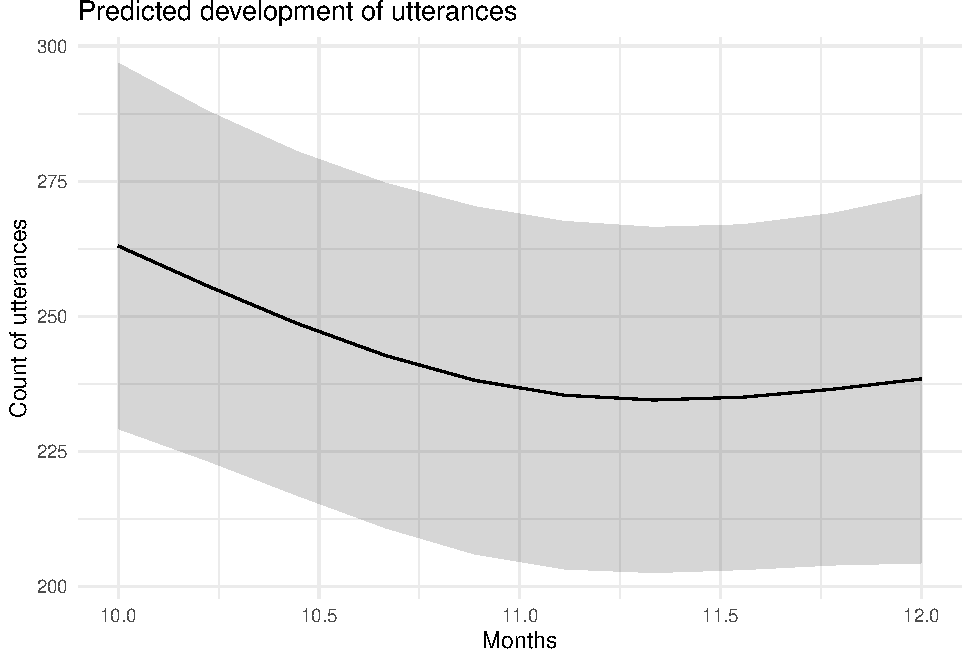
\includegraphics{supplement_files/figure-latex/utter-gam-2-plot-1.pdf}

\hypertarget{contingent-talks-development}{%
\subsection{Contingent talks
development}\label{contingent-talks-development}}

\begin{Shaded}
\begin{Highlighting}[]
\NormalTok{all_tot }\OperatorTok
\StringTok{  }\KeywordTok{ggplot}\NormalTok{(}\KeywordTok{aes}\NormalTok{(ct)) }\OperatorTok{+}\StringTok{ }\KeywordTok{geom_density}\NormalTok{() }\OperatorTok{+}\StringTok{ }\KeywordTok{geom_rug}\NormalTok{(}\DataTypeTok{alpha =} \FloatTok{0.1}\NormalTok{) }\OperatorTok{+}
\StringTok{  }\KeywordTok{labs}\NormalTok{(}
    \DataTypeTok{title =} \StringTok{"Distribution of the count of CTs"}\NormalTok{,}
    \DataTypeTok{x =} \StringTok{"Count of maternal CTs"}
\NormalTok{  )}
\end{Highlighting}
\end{Shaded}

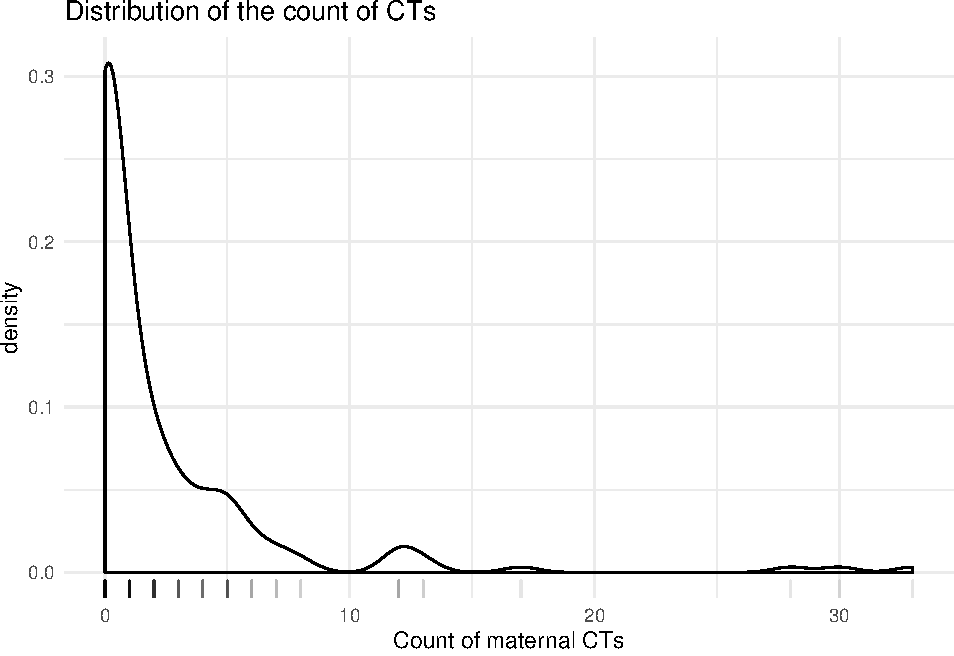
\includegraphics{supplement_files/figure-latex/ct-1.pdf}

\begin{center}\rule{0.5\linewidth}{\linethickness}\end{center}

The following models test cultural group.

\begin{Shaded}
\begin{Highlighting}[]
\NormalTok{ct_nb <-}\StringTok{ }\KeywordTok{glm.nb}\NormalTok{(ct }\OperatorTok{~}\StringTok{ }\NormalTok{months, }\DataTypeTok{data =}\NormalTok{ all_tot)}
\NormalTok{theta_}\DecValTok{4}\NormalTok{ <-}\StringTok{ }\KeywordTok{summary}\NormalTok{(ct_nb)[[}\StringTok{"theta"}\NormalTok{]]}

\NormalTok{ct_gam <-}\StringTok{ }\KeywordTok{gam}\NormalTok{(}
\NormalTok{  ct }\OperatorTok{~}
\StringTok{    }\NormalTok{back_o }\OperatorTok{+}
\StringTok{    }\KeywordTok{s}\NormalTok{(months, }\DataTypeTok{k =} \DecValTok{3}\NormalTok{) }\OperatorTok{+}
\StringTok{    }\KeywordTok{s}\NormalTok{(months, }\DataTypeTok{k =} \DecValTok{3}\NormalTok{, }\DataTypeTok{by =}\NormalTok{ back_o) }\OperatorTok{+}
\StringTok{    }\KeywordTok{s}\NormalTok{(months, dyad, }\DataTypeTok{k =} \DecValTok{2}\NormalTok{, }\DataTypeTok{bs =} \StringTok{"fs"}\NormalTok{, }\DataTypeTok{m =} \DecValTok{1}\NormalTok{),}
  \DataTypeTok{data =}\NormalTok{ all_tot,}
  \DataTypeTok{method =} \StringTok{"ML"}\NormalTok{,}
  \DataTypeTok{family =} \KeywordTok{negbin}\NormalTok{(theta_}\DecValTok{4}\NormalTok{)}
\NormalTok{)}
\end{Highlighting}
\end{Shaded}

\begin{verbatim}
## Warning in gam.side(sm, X, tol = .Machine$double.eps^0.5): model has
## repeated 1-d smooths of same variable.
\end{verbatim}

\begin{Shaded}
\begin{Highlighting}[]
\KeywordTok{summary}\NormalTok{(ct_gam)}
\end{Highlighting}
\end{Shaded}

\begin{verbatim}
## 
## Family: Negative Binomial(0.385) 
## Link function: log 
## 
## Formula:
## ct ~ back_o + s(months, k = 3) + s(months, k = 3, by = back_o) + 
##     s(months, dyad, k = 2, bs = "fs", m = 1)
## 
## Parametric coefficients:
##               Estimate Std. Error z value Pr(>|z|)  
## (Intercept)     0.6527     0.2977   2.192   0.0283 *
## back_oBengali  -0.9863     0.4347  -2.269   0.0233 *
## back_oChinese  -0.2083     0.4226  -0.493   0.6222  
## ---
## Signif. codes:  0 '***' 0.001 '**' 0.01 '*' 0.05 '.' 0.1 ' ' 1
## 
## Approximate significance of smooth terms:
##                           edf  Ref.df Chi.sq p-value   
## s(months)                1.00   1.000  3.039 0.08129 . 
## s(months):back_oBengali  1.75   1.937  3.064 0.24022   
## s(months):back_oChinese  1.00   1.000  0.391 0.53191   
## s(months,dyad)          18.38 112.000 27.602 0.00937 **
## ---
## Signif. codes:  0 '***' 0.001 '**' 0.01 '*' 0.05 '.' 0.1 ' ' 1
## 
## R-sq.(adj) =  0.394   Deviance explained = 43.7%
## -ML = 315.49  Scale est. = 1         n = 172
\end{verbatim}

\begin{Shaded}
\begin{Highlighting}[]
\NormalTok{ct_gam_null <-}\StringTok{ }\KeywordTok{gam}\NormalTok{(}
\NormalTok{  ct }\OperatorTok{~}
\StringTok{    }\CommentTok{# back_o +}
\StringTok{    }\KeywordTok{s}\NormalTok{(months, }\DataTypeTok{k =} \DecValTok{3}\NormalTok{) }\OperatorTok{+}
\StringTok{    }\CommentTok{# s(months, k = 3, by = back_o) +}
\StringTok{    }\KeywordTok{s}\NormalTok{(months, dyad, }\DataTypeTok{k =} \DecValTok{2}\NormalTok{, }\DataTypeTok{bs =} \StringTok{"fs"}\NormalTok{, }\DataTypeTok{m =} \DecValTok{1}\NormalTok{),}
  \DataTypeTok{data =}\NormalTok{ all_tot,}
  \DataTypeTok{method =} \StringTok{"ML"}\NormalTok{,}
  \DataTypeTok{family =} \KeywordTok{negbin}\NormalTok{(theta_}\DecValTok{4}\NormalTok{)}
\NormalTok{)}
\end{Highlighting}
\end{Shaded}

\begin{verbatim}
## Warning in gam.side(sm, X, tol = .Machine$double.eps^0.5): model has
## repeated 1-d smooths of same variable.
\end{verbatim}

\begin{Shaded}
\begin{Highlighting}[]
\KeywordTok{compareML}\NormalTok{(ct_gam_null, ct_gam)}
\end{Highlighting}
\end{Shaded}

\begin{verbatim}
## ct_gam_null: ct ~ s(months, k = 3) + s(months, dyad, k = 2, bs = "fs", m = 1)
## 
## ct_gam: ct ~ back_o + s(months, k = 3) + s(months, k = 3, by = back_o) + 
##     s(months, dyad, k = 2, bs = "fs", m = 1)
## 
## Chi-square test of ML scores
## -----
##         Model    Score Edf Difference    Df p.value Sig.
## 1 ct_gam_null 318.9134   5                              
## 2      ct_gam 315.4851  11      3.428 6.000   0.334     
## 
## AIC difference: 0.60, model ct_gam has lower AIC.
\end{verbatim}

\begin{verbatim}
## Warning in compareML(ct_gam_null, ct_gam): Only small difference in ML...
\end{verbatim}

\begin{Shaded}
\begin{Highlighting}[]
\KeywordTok{plot_smooths}\NormalTok{(ct_gam, months, }\DataTypeTok{facet_terms =}\NormalTok{ back_o, }\DataTypeTok{series_length =} \DecValTok{10}\NormalTok{, }\DataTypeTok{transform =}\NormalTok{ exp) }\OperatorTok{+}
\StringTok{  }\KeywordTok{labs}\NormalTok{(}\DataTypeTok{x =} \StringTok{"Months"}\NormalTok{, }\DataTypeTok{y =} \StringTok{"Count of CTs"}\NormalTok{, }\DataTypeTok{title =} \StringTok{"Predicted development of CTs by background"}\NormalTok{)}
\end{Highlighting}
\end{Shaded}

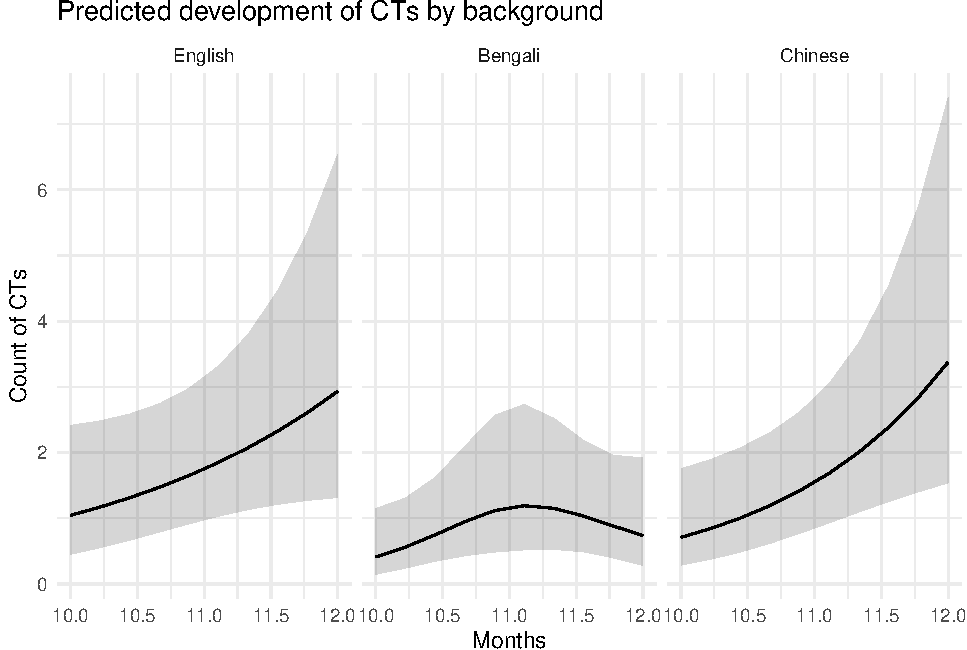
\includegraphics{supplement_files/figure-latex/ct-gam-plot-1.pdf}

\begin{center}\rule{0.5\linewidth}{\linethickness}\end{center}

The following models test time sample.

\begin{Shaded}
\begin{Highlighting}[]
\NormalTok{ct_gam_}\DecValTok{2}\NormalTok{ <-}\StringTok{ }\KeywordTok{gam}\NormalTok{(}
\NormalTok{  count }\OperatorTok{~}
\StringTok{    }\KeywordTok{s}\NormalTok{(months, }\DataTypeTok{k =} \DecValTok{3}\NormalTok{) }\OperatorTok{+}
\StringTok{    }\KeywordTok{s}\NormalTok{(months, dyad, }\DataTypeTok{k =} \DecValTok{2}\NormalTok{, }\DataTypeTok{bs =} \StringTok{"fs"}\NormalTok{, }\DataTypeTok{m =} \DecValTok{1}\NormalTok{),}
  \DataTypeTok{data =}\NormalTok{ all_tot,}
  \DataTypeTok{method =} \StringTok{"ML"}\NormalTok{,}
  \DataTypeTok{family =} \KeywordTok{negbin}\NormalTok{(theta_}\DecValTok{4}\NormalTok{)}
\NormalTok{)}
\end{Highlighting}
\end{Shaded}

\begin{verbatim}
## Warning in gam.side(sm, X, tol = .Machine$double.eps^0.5): model has
## repeated 1-d smooths of same variable.
\end{verbatim}

\begin{Shaded}
\begin{Highlighting}[]
\NormalTok{ct_gam_}\DecValTok{2}\NormalTok{_null <-}\StringTok{ }\KeywordTok{gam}\NormalTok{(}
\NormalTok{  count }\OperatorTok{~}
\StringTok{    }\CommentTok{# s(months, k = 3) +}
\StringTok{    }\KeywordTok{s}\NormalTok{(months, dyad, }\DataTypeTok{k =} \DecValTok{2}\NormalTok{, }\DataTypeTok{bs =} \StringTok{"fs"}\NormalTok{, }\DataTypeTok{m =} \DecValTok{1}\NormalTok{),}
  \DataTypeTok{data =}\NormalTok{ all_tot,}
  \DataTypeTok{method =} \StringTok{"ML"}\NormalTok{,}
  \DataTypeTok{family =} \KeywordTok{negbin}\NormalTok{(theta_}\DecValTok{4}\NormalTok{)}
\NormalTok{)}

\KeywordTok{compareML}\NormalTok{(ct_gam_}\DecValTok{2}\NormalTok{_null, ct_gam_}\DecValTok{2}\NormalTok{)}
\end{Highlighting}
\end{Shaded}

\begin{verbatim}
## ct_gam_2_null: count ~ s(months, dyad, k = 2, bs = "fs", m = 1)
## 
## ct_gam_2: count ~ s(months, k = 3) + s(months, dyad, k = 2, bs = "fs", 
##     m = 1)
## 
## Chi-square test of ML scores
## -----
##           Model    Score Edf Difference    Df p.value Sig.
## 1 ct_gam_2_null 641.7134   3                              
## 2      ct_gam_2 637.2323   5      4.481 2.000   0.011  *  
## 
## AIC difference: 6.96, model ct_gam_2 has lower AIC.
\end{verbatim}

\begin{verbatim}
## Warning in compareML(ct_gam_2_null, ct_gam_2): Only small difference in ML...
\end{verbatim}

\begin{Shaded}
\begin{Highlighting}[]
\KeywordTok{plot_smooths}\NormalTok{(ct_gam_}\DecValTok{2}\NormalTok{, months, }\DataTypeTok{series_length =} \DecValTok{10}\NormalTok{, }\DataTypeTok{transform =}\NormalTok{ exp) }\OperatorTok{+}
\StringTok{  }\KeywordTok{labs}\NormalTok{(}\DataTypeTok{x =} \StringTok{"Months"}\NormalTok{, }\DataTypeTok{y =} \StringTok{"Count of CTs"}\NormalTok{, }\DataTypeTok{title =} \StringTok{"Predicted development of CTs"}\NormalTok{)}
\end{Highlighting}
\end{Shaded}

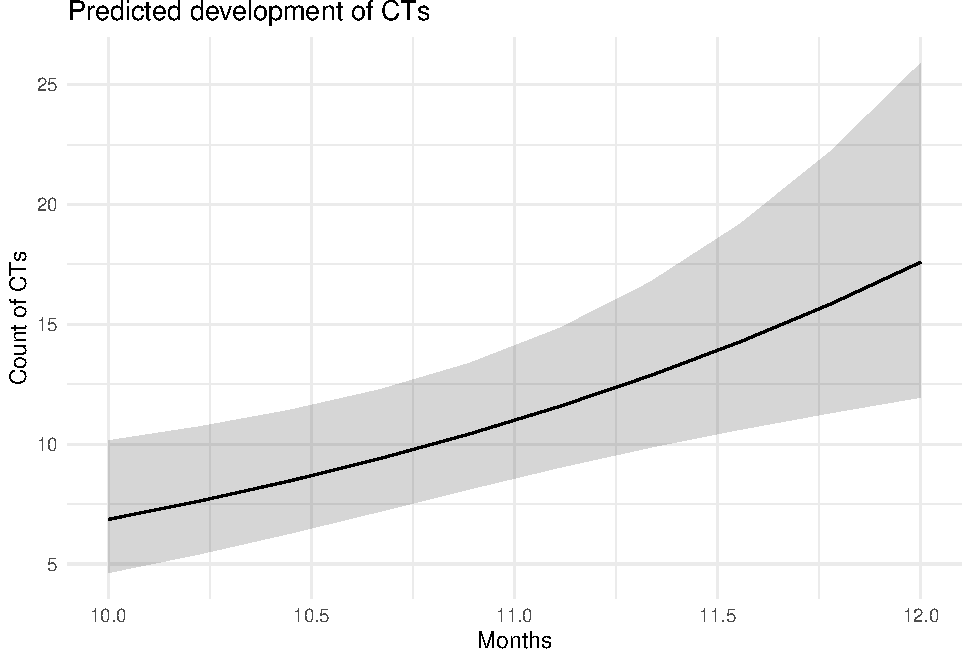
\includegraphics{supplement_files/figure-latex/ct-gam-2-plot-1.pdf}

\newpage

\hypertarget{analysis-1c.-predictors-of-pointing}{%
\section{Analysis 1c. Predictors of
pointing}\label{analysis-1c.-predictors-of-pointing}}

The following GLMMs test the relation between pointing and reaches/HoGs.
The count of pointing refers to the one produced by the infant in the
subsequent session: For example, the count of reaches at 10 months is
matched with the count of points at 11 months, and that of reaches at 11
months is matched with the count of points at 12 months. This allows us
to test whether gestures at a certain sampling time predict the
production of pointing at the next sampling time. Data on pointing at 10
months is dropped, since there is no data on gestures prior to 10
months.

\hypertarget{reaches}{%
\subsection{Reaches}\label{reaches}}

\begin{Shaded}
\begin{Highlighting}[]
\NormalTok{reach_point_lead_nb <-}\StringTok{ }\KeywordTok{glm.nb}\NormalTok{(lead_point }\OperatorTok{~}\StringTok{ }\NormalTok{reach, }\DataTypeTok{data =}\NormalTok{ reach_point_lead)}
\NormalTok{theta_}\DecValTok{5}\NormalTok{ <-}\StringTok{ }\KeywordTok{summary}\NormalTok{(reach_point_lead_nb)[[}\StringTok{"theta"}\NormalTok{]]}

\NormalTok{reach_point_lm <-}\StringTok{ }\KeywordTok{glmer}\NormalTok{(}
\NormalTok{  lead_point }\OperatorTok{~}
\StringTok{    }\NormalTok{reach }\OperatorTok{*}
\StringTok{    }\NormalTok{background }\OperatorTok{+}
\StringTok{    }\NormalTok{(}\DecValTok{1}\OperatorTok{|}\NormalTok{dyad),}
  \DataTypeTok{data =}\NormalTok{ reach_point_lead,}
  \DataTypeTok{family =} \KeywordTok{negbin}\NormalTok{(theta_}\DecValTok{5}\NormalTok{)}
\NormalTok{)}
\KeywordTok{summary}\NormalTok{(reach_point_lm)}
\end{Highlighting}
\end{Shaded}

\begin{verbatim}
## Generalized linear mixed model fit by maximum likelihood (Laplace
##   Approximation) [glmerMod]
##  Family: Negative Binomial(0.268)  ( log )
## Formula: lead_point ~ reach * background + (1 | dyad)
##    Data: reach_point_lead
## 
##      AIC      BIC   logLik deviance df.resid 
##    523.3    545.1   -253.7    507.3      104 
## 
## Scaled residuals: 
##     Min      1Q  Median      3Q     Max 
## -0.5066 -0.4983 -0.3934  0.1438  3.0193 
## 
## Random effects:
##  Groups Name        Variance Std.Dev.
##  dyad   (Intercept) 0.157    0.3963  
## Number of obs: 112, groups:  dyad, 57
## 
## Fixed effects:
##                         Estimate Std. Error z value Pr(>|z|)
## (Intercept)              0.72148    0.60137   1.200    0.230
## reach                    0.06137    0.09716   0.632    0.528
## backgroundChinese        1.10780    0.72839   1.521    0.128
## backgroundEnglish        0.84351    0.68166   1.237    0.216
## reach:backgroundChinese -0.24685    0.16104  -1.533    0.125
## reach:backgroundEnglish -0.08717    0.13746  -0.634    0.526
## 
## Correlation of Fixed Effects:
##             (Intr) reach  bckgrC bckgrE rch:bC
## reach       -0.724                            
## bckgrndChns -0.709  0.550                     
## bckgrndEngl -0.558  0.506  0.508              
## rch:bckgrnC  0.453 -0.610 -0.710 -0.298       
## rch:bckgrnE  0.449 -0.681 -0.366 -0.599  0.412
\end{verbatim}

\begin{Shaded}
\begin{Highlighting}[]
\KeywordTok{plot_model}\NormalTok{(reach_point_lm, }\DataTypeTok{type =} \StringTok{"pred"}\NormalTok{, }\DataTypeTok{terms =} \KeywordTok{c}\NormalTok{(}\StringTok{"reach"}\NormalTok{, }\StringTok{"background"}\NormalTok{))}
\end{Highlighting}
\end{Shaded}

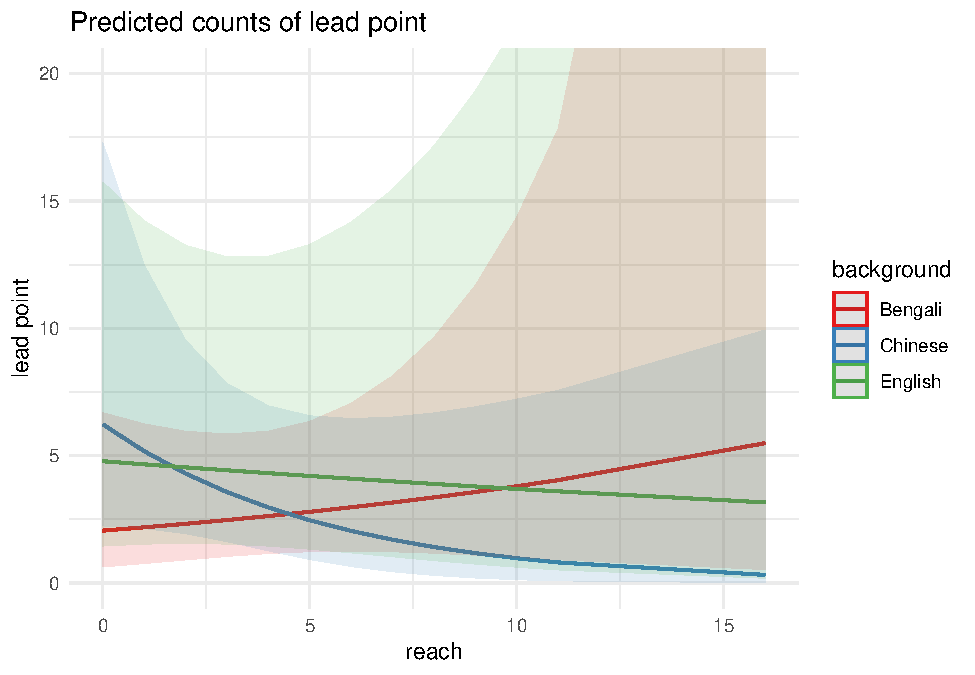
\includegraphics{supplement_files/figure-latex/reach-point-plot-1.pdf}

\hypertarget{hogs}{%
\subsection{HoGs}\label{hogs}}

\begin{Shaded}
\begin{Highlighting}[]
\NormalTok{hg_point_lead_nb <-}\StringTok{ }\KeywordTok{glm.nb}\NormalTok{(lead_point }\OperatorTok{~}\StringTok{ }\NormalTok{ho_gv, }\DataTypeTok{data =} \KeywordTok{filter}\NormalTok{(hg_point_lead, ho_gv }\OperatorTok{<}\StringTok{ }\DecValTok{20}\NormalTok{))}
\NormalTok{theta_}\DecValTok{6}\NormalTok{ <-}\StringTok{ }\KeywordTok{summary}\NormalTok{(reach_point_lead_nb)[[}\StringTok{"theta"}\NormalTok{]]}

\NormalTok{hg_point_lm <-}\StringTok{ }\KeywordTok{glmer}\NormalTok{(}
\NormalTok{  lead_point }\OperatorTok{~}
\StringTok{    }\NormalTok{ho_gv }\OperatorTok{*}
\StringTok{    }\NormalTok{background }\OperatorTok{+}
\StringTok{    }\NormalTok{(}\DecValTok{1}\OperatorTok{|}\NormalTok{dyad),}
  \DataTypeTok{data =} \KeywordTok{filter}\NormalTok{(hg_point_lead, ho_gv }\OperatorTok{<}\StringTok{ }\DecValTok{20}\NormalTok{),}
  \DataTypeTok{family =} \KeywordTok{negbin}\NormalTok{(theta_}\DecValTok{6}\NormalTok{)}
\NormalTok{)}
\end{Highlighting}
\end{Shaded}

\begin{verbatim}
## boundary (singular) fit: see ?isSingular
\end{verbatim}

\begin{Shaded}
\begin{Highlighting}[]
\KeywordTok{summary}\NormalTok{(hg_point_lm)}
\end{Highlighting}
\end{Shaded}

\begin{verbatim}
## Generalized linear mixed model fit by maximum likelihood (Laplace
##   Approximation) [glmerMod]
##  Family: Negative Binomial(0.268)  ( log )
## Formula: lead_point ~ ho_gv * background + (1 | dyad)
##    Data: filter(hg_point_lead, ho_gv < 20)
## 
##      AIC      BIC   logLik deviance df.resid 
##    503.6    525.1   -243.8    487.6      101 
## 
## Scaled residuals: 
##     Min      1Q  Median      3Q     Max 
## -0.5152 -0.5009 -0.4033  0.1257  6.1781 
## 
## Random effects:
##  Groups Name        Variance  Std.Dev. 
##  dyad   (Intercept) 1.407e-10 1.186e-05
## Number of obs: 109, groups:  dyad, 57
## 
## Fixed effects:
##                         Estimate Std. Error z value Pr(>|z|)   
## (Intercept)              1.37535    0.45787   3.004  0.00267 **
## ho_gv                   -0.10720    0.07934  -1.351  0.17665   
## backgroundChinese        0.11398    0.67981   0.168  0.86685   
## backgroundEnglish       -0.22597    0.62061  -0.364  0.71577   
## ho_gv:backgroundChinese  0.12681    0.13692   0.926  0.35435   
## ho_gv:backgroundEnglish  0.31874    0.15354   2.076  0.03790 * 
## ---
## Signif. codes:  0 '***' 0.001 '**' 0.01 '*' 0.05 '.' 0.1 ' ' 1
## 
## Correlation of Fixed Effects:
##             (Intr) ho_gv  bckgrC bckgrE h_gv:C
## ho_gv       -0.681                            
## bckgrndChns -0.674  0.459                     
## bckgrndEngl -0.738  0.502  0.497              
## h_gv:bckgrC  0.395 -0.579 -0.714 -0.291       
## h_gv:bckgrE  0.352 -0.517 -0.237 -0.621  0.299
## convergence code: 0
## boundary (singular) fit: see ?isSingular
\end{verbatim}

\begin{Shaded}
\begin{Highlighting}[]
\KeywordTok{plot_model}\NormalTok{(hg_point_lm, }\DataTypeTok{type =} \StringTok{"pred"}\NormalTok{, }\DataTypeTok{terms =} \KeywordTok{c}\NormalTok{(}\StringTok{"ho_gv"}\NormalTok{, }\StringTok{"background"}\NormalTok{))}
\end{Highlighting}
\end{Shaded}

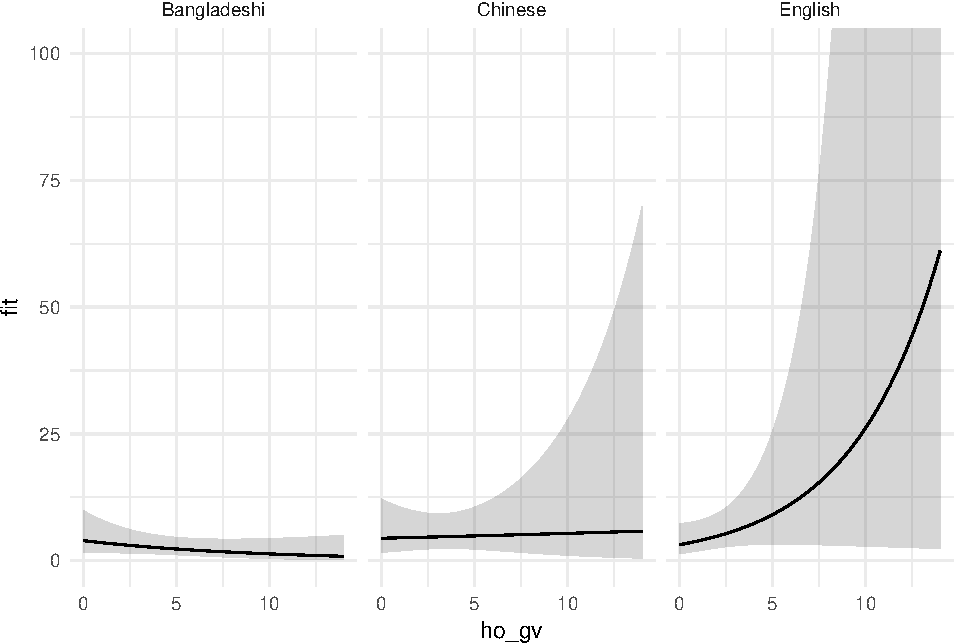
\includegraphics{supplement_files/figure-latex/hg-point-plot-1.pdf}

\newpage

\hypertarget{analysis-2.-predictors-of-vocabulary-scores-at-12-and-18-months}{%
\section{Analysis 2. Predictors of vocabulary scores at 12 and 18
months}\label{analysis-2.-predictors-of-vocabulary-scores-at-12-and-18-months}}

\hypertarget{comprehension-at-12-and-18-months}{%
\subsection{Comprehension at 12 and 18
months}\label{comprehension-at-12-and-18-months}}

\hypertarget{all-gestures-combined}{%
\subsubsection{All gestures combined}\label{all-gestures-combined}}

\begin{Shaded}
\begin{Highlighting}[]
\NormalTok{all_gest_lm <-}\StringTok{ }\KeywordTok{glm}\NormalTok{(}
\NormalTok{  comprehension }\OperatorTok{~}
\StringTok{    }\NormalTok{count_tot }\OperatorTok{*}
\StringTok{    }\NormalTok{months }\OperatorTok{*}
\StringTok{    }\NormalTok{background,}
  \DataTypeTok{data =}\NormalTok{ vocab,}
  \DataTypeTok{family =}\NormalTok{ poisson}
\NormalTok{)}
\KeywordTok{summary}\NormalTok{(all_gest_lm)}
\end{Highlighting}
\end{Shaded}

\begin{verbatim}
## 
## Call:
## glm(formula = comprehension ~ count_tot * months * background, 
##     family = poisson, data = vocab)
## 
## Deviance Residuals: 
##     Min       1Q   Median       3Q      Max  
## -12.534   -3.589   -0.588    2.339   16.033  
## 
## Coefficients:
##                                        Estimate Std. Error z value
## (Intercept)                           4.6615113  0.0323369 144.155
## count_tot                            -0.0048625  0.0007949  -6.117
## months18                              0.6528243  0.0389823  16.747
## backgroundBengali                     0.0635196  0.0586909   1.082
## backgroundChinese                    -0.8899846  0.0570165 -15.609
## count_tot:months18                    0.0068861  0.0008836   7.793
## count_tot:backgroundBengali           0.0017305  0.0013854   1.249
## count_tot:backgroundChinese           0.0226132  0.0010689  21.155
## months18:backgroundBengali           -0.2163911  0.0726471  -2.979
## months18:backgroundChinese            0.6034030  0.0675504   8.933
## count_tot:months18:backgroundBengali -0.0016836  0.0016536  -1.018
## count_tot:months18:backgroundChinese -0.0157740  0.0012443 -12.677
##                                      Pr(>|z|)    
## (Intercept)                           < 2e-16 ***
## count_tot                            9.53e-10 ***
## months18                              < 2e-16 ***
## backgroundBengali                      0.2791    
## backgroundChinese                     < 2e-16 ***
## count_tot:months18                   6.52e-15 ***
## count_tot:backgroundBengali            0.2116    
## count_tot:backgroundChinese           < 2e-16 ***
## months18:backgroundBengali             0.0029 ** 
## months18:backgroundChinese            < 2e-16 ***
## count_tot:months18:backgroundBengali   0.3086    
## count_tot:months18:backgroundChinese  < 2e-16 ***
## ---
## Signif. codes:  0 '***' 0.001 '**' 0.01 '*' 0.05 '.' 0.1 ' ' 1
## 
## (Dispersion parameter for poisson family taken to be 1)
## 
##     Null deviance: 6642.1  on 108  degrees of freedom
## Residual deviance: 3326.7  on  97  degrees of freedom
##   (11 observations deleted due to missingness)
## AIC: 4072.7
## 
## Number of Fisher Scoring iterations: 5
\end{verbatim}

\begin{Shaded}
\begin{Highlighting}[]
\KeywordTok{plot_model}\NormalTok{(all_gest_lm, }\DataTypeTok{type =} \StringTok{"pred"}\NormalTok{, }\DataTypeTok{terms =} \KeywordTok{c}\NormalTok{(}\StringTok{"count_tot"}\NormalTok{, }\StringTok{"months"}\NormalTok{, }\StringTok{"background"}\NormalTok{))}
\end{Highlighting}
\end{Shaded}

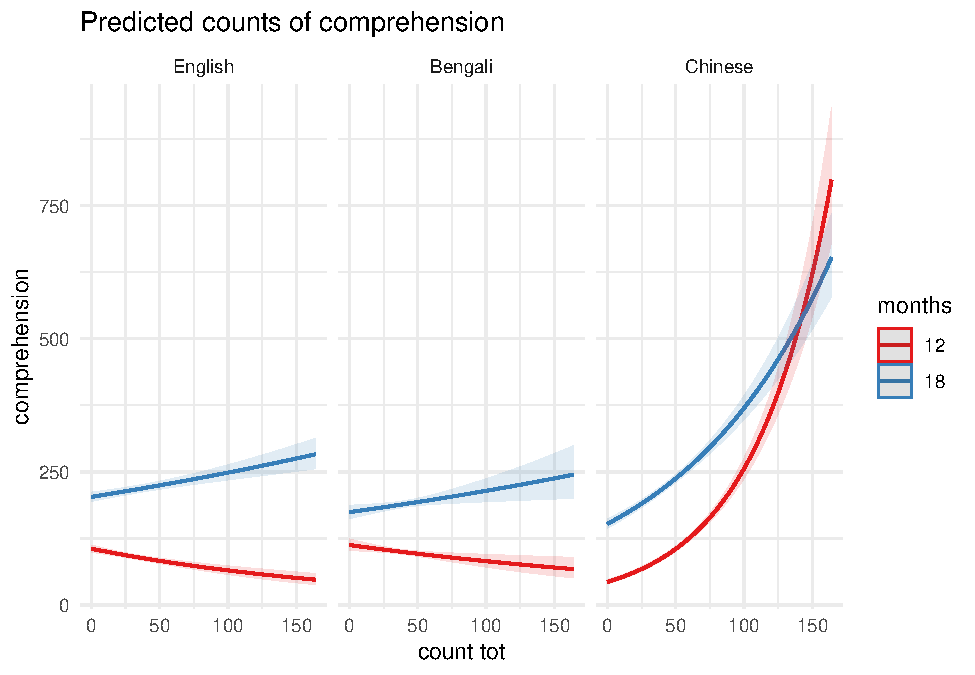
\includegraphics{supplement_files/figure-latex/all-gest-lm-plot-1.pdf}

\hypertarget{hogs-points}{%
\subsubsection{HoGs + points}\label{hogs-points}}

\begin{Shaded}
\begin{Highlighting}[]
\NormalTok{hgp_lm <-}\StringTok{ }\KeywordTok{glm}\NormalTok{(}
\NormalTok{  comprehension }\OperatorTok{~}
\StringTok{    }\NormalTok{hgp_tot }\OperatorTok{*}
\StringTok{    }\NormalTok{months }\OperatorTok{*}
\StringTok{    }\NormalTok{background,}
  \DataTypeTok{data =}\NormalTok{ vocab,}
  \DataTypeTok{family =} \KeywordTok{poisson}\NormalTok{()}
\NormalTok{)}
\KeywordTok{summary}\NormalTok{(hgp_lm)}
\end{Highlighting}
\end{Shaded}

\begin{verbatim}
## 
## Call:
## glm(formula = comprehension ~ hgp_tot * months * background, 
##     family = poisson(), data = vocab)
## 
## Deviance Residuals: 
##      Min        1Q    Median        3Q       Max  
## -12.0912   -4.0304   -0.3296    2.6629   17.5976  
## 
## Coefficients:
##                                      Estimate Std. Error z value Pr(>|z|)
## (Intercept)                         4.6377993  0.0292714 158.441  < 2e-16
## hgp_tot                            -0.0053955  0.0008347  -6.464 1.02e-10
## months18                            0.6962163  0.0354287  19.651  < 2e-16
## backgroundBengali                   0.0003589  0.0522614   0.007  0.99452
## backgroundChinese                  -0.6535607  0.0506378 -12.907  < 2e-16
## hgp_tot:months18                    0.0072361  0.0009178   7.885 3.16e-15
## hgp_tot:backgroundBengali           0.0041596  0.0015628   2.662  0.00778
## hgp_tot:backgroundChinese           0.0218970  0.0011069  19.782  < 2e-16
## months18:backgroundBengali         -0.1927418  0.0644893  -2.989  0.00280
## months18:backgroundChinese          0.4461919  0.0600587   7.429 1.09e-13
## hgp_tot:months18:backgroundBengali -0.0024355  0.0018614  -1.308  0.19074
## hgp_tot:months18:backgroundChinese -0.0154648  0.0012786 -12.095  < 2e-16
##                                       
## (Intercept)                        ***
## hgp_tot                            ***
## months18                           ***
## backgroundBengali                     
## backgroundChinese                  ***
## hgp_tot:months18                   ***
## hgp_tot:backgroundBengali          ** 
## hgp_tot:backgroundChinese          ***
## months18:backgroundBengali         ** 
## months18:backgroundChinese         ***
## hgp_tot:months18:backgroundBengali    
## hgp_tot:months18:backgroundChinese ***
## ---
## Signif. codes:  0 '***' 0.001 '**' 0.01 '*' 0.05 '.' 0.1 ' ' 1
## 
## (Dispersion parameter for poisson family taken to be 1)
## 
##     Null deviance: 6642.1  on 108  degrees of freedom
## Residual deviance: 3459.2  on  97  degrees of freedom
##   (11 observations deleted due to missingness)
## AIC: 4205.2
## 
## Number of Fisher Scoring iterations: 5
\end{verbatim}

\begin{Shaded}
\begin{Highlighting}[]
\KeywordTok{plot_model}\NormalTok{(hgp_lm, }\DataTypeTok{type =} \StringTok{"pred"}\NormalTok{, }\DataTypeTok{terms =} \KeywordTok{c}\NormalTok{(}\StringTok{"hgp_tot"}\NormalTok{, }\StringTok{"months"}\NormalTok{, }\StringTok{"background"}\NormalTok{))}
\end{Highlighting}
\end{Shaded}

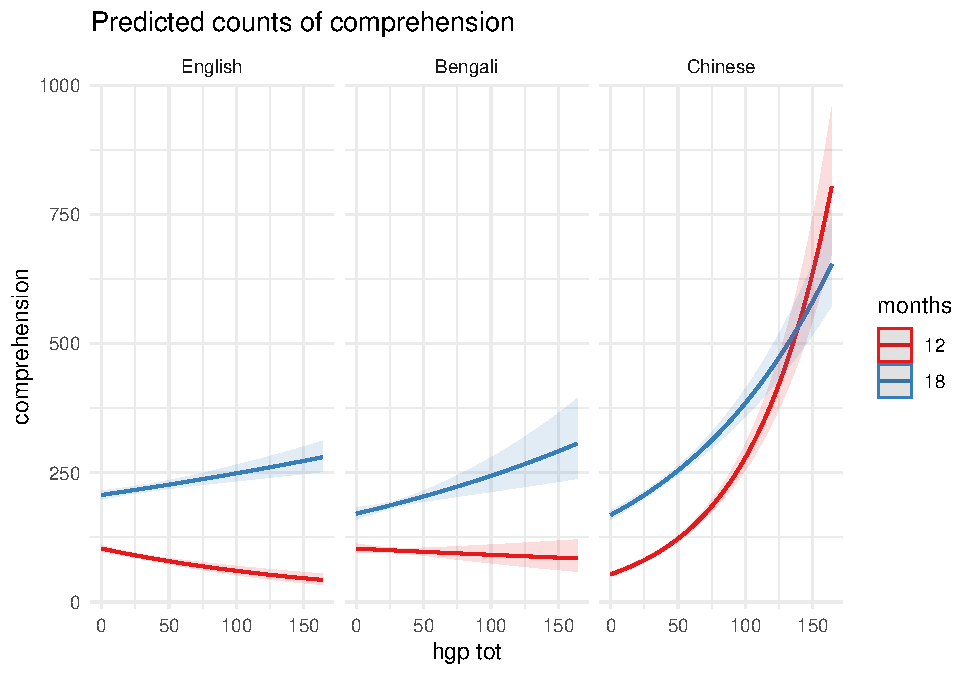
\includegraphics{supplement_files/figure-latex/hgp-lm-2-plot-1.pdf}

\hypertarget{reaches-1}{%
\subsubsection{Reaches}\label{reaches-1}}

\begin{Shaded}
\begin{Highlighting}[]
\NormalTok{reach_lm <-}\StringTok{ }\KeywordTok{glm}\NormalTok{(}
\NormalTok{  comprehension }\OperatorTok{~}
\StringTok{    }\NormalTok{reach_tot }\OperatorTok{*}
\StringTok{    }\NormalTok{months }\OperatorTok{*}
\StringTok{    }\NormalTok{background,}
  \DataTypeTok{data =}\NormalTok{ vocab,}
  \DataTypeTok{family =} \KeywordTok{poisson}\NormalTok{()}
\NormalTok{)}
\KeywordTok{summary}\NormalTok{(reach_lm)}
\end{Highlighting}
\end{Shaded}

\begin{verbatim}
## 
## Call:
## glm(formula = comprehension ~ reach_tot * months * background, 
##     family = poisson(), data = vocab)
## 
## Deviance Residuals: 
##      Min        1Q    Median        3Q       Max  
## -15.0397   -4.2179   -0.4216    3.4316   17.2738  
## 
## Coefficients:
##                                       Estimate Std. Error z value Pr(>|z|)
## (Intercept)                           4.456258   0.036398 122.433  < 2e-16
## reach_tot                             0.008853   0.003627   2.441  0.01465
## months18                              0.892274   0.043543  20.492  < 2e-16
## backgroundBengali                     0.384841   0.057007   6.751 1.47e-11
## backgroundChinese                    -0.308676   0.060521  -5.100 3.39e-07
## reach_tot:months18                   -0.003657   0.004337  -0.843  0.39916
## reach_tot:backgroundBengali          -0.030842   0.005119  -6.024 1.70e-09
## reach_tot:backgroundChinese           0.042672   0.005541   7.701 1.35e-14
## months18:backgroundBengali           -0.424152   0.069985  -6.061 1.36e-09
## months18:backgroundChinese            0.187235   0.071705   2.611  0.00902
## reach_tot:months18:backgroundBengali  0.019788   0.006201   3.191  0.00142
## reach_tot:months18:backgroundChinese -0.026341   0.006649  -3.961 7.45e-05
##                                         
## (Intercept)                          ***
## reach_tot                            *  
## months18                             ***
## backgroundBengali                    ***
## backgroundChinese                    ***
## reach_tot:months18                      
## reach_tot:backgroundBengali          ***
## reach_tot:backgroundChinese          ***
## months18:backgroundBengali           ***
## months18:backgroundChinese           ** 
## reach_tot:months18:backgroundBengali ** 
## reach_tot:months18:backgroundChinese ***
## ---
## Signif. codes:  0 '***' 0.001 '**' 0.01 '*' 0.05 '.' 0.1 ' ' 1
## 
## (Dispersion parameter for poisson family taken to be 1)
## 
##     Null deviance: 6642.1  on 108  degrees of freedom
## Residual deviance: 4011.7  on  97  degrees of freedom
##   (11 observations deleted due to missingness)
## AIC: 4757.8
## 
## Number of Fisher Scoring iterations: 5
\end{verbatim}

\begin{Shaded}
\begin{Highlighting}[]
\KeywordTok{plot_model}\NormalTok{(reach_lm, }\DataTypeTok{type =} \StringTok{"pred"}\NormalTok{, }\DataTypeTok{terms =} \KeywordTok{c}\NormalTok{(}\StringTok{"reach_tot"}\NormalTok{, }\StringTok{"months"}\NormalTok{, }\StringTok{"background"}\NormalTok{))}
\end{Highlighting}
\end{Shaded}

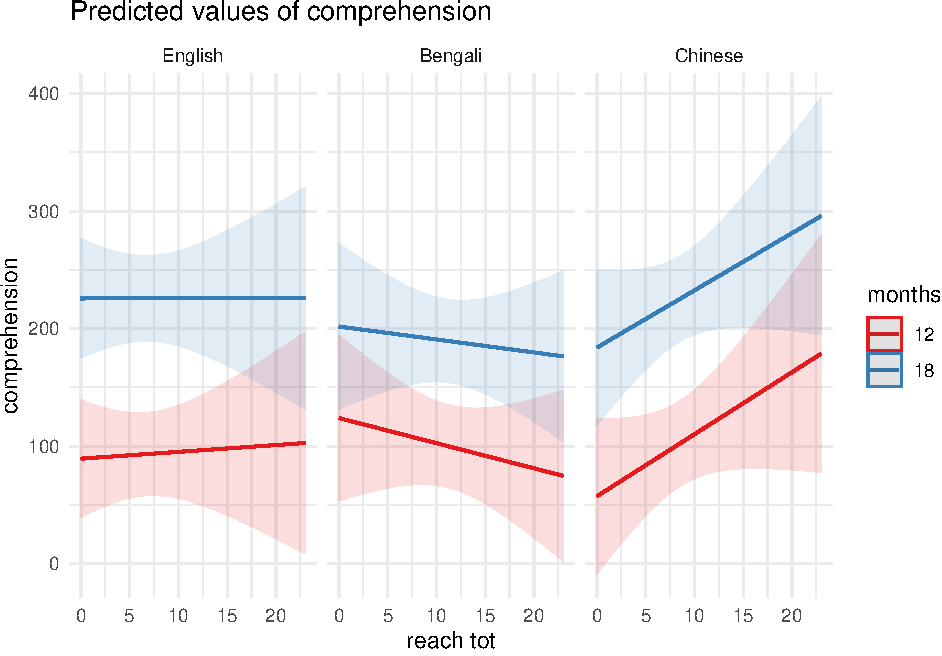
\includegraphics{supplement_files/figure-latex/reach-lm-2-plot-1.pdf}

\hypertarget{maternal-utterances}{%
\subsubsection{Maternal utterances}\label{maternal-utterances}}

\begin{Shaded}
\begin{Highlighting}[]
\NormalTok{utt_lm <-}\StringTok{ }\KeywordTok{glm}\NormalTok{(}
\NormalTok{  comprehension }\OperatorTok{~}
\StringTok{    }\NormalTok{utt_tot }\OperatorTok{*}
\StringTok{    }\NormalTok{months }\OperatorTok{*}
\StringTok{    }\NormalTok{background,}
  \DataTypeTok{data =}\NormalTok{ vocab,}
  \DataTypeTok{family =} \KeywordTok{poisson}\NormalTok{()}
\NormalTok{)}
\KeywordTok{summary}\NormalTok{(utt_lm)}
\end{Highlighting}
\end{Shaded}

\begin{verbatim}
## 
## Call:
## glm(formula = comprehension ~ utt_tot * months * background, 
##     family = poisson(), data = vocab)
## 
## Deviance Residuals: 
##     Min       1Q   Median       3Q      Max  
## -14.146   -4.714   -1.202    3.528   16.309  
## 
## Coefficients:
##                                      Estimate Std. Error z value Pr(>|z|)
## (Intercept)                         6.1169916  0.1184273  51.652  < 2e-16
## utt_tot                            -0.0018179  0.0001481 -12.277  < 2e-16
## months18                           -0.1830862  0.1463324  -1.251    0.211
## backgroundBengali                  -1.6180843  0.1253368 -12.910  < 2e-16
## backgroundChinese                  -1.9734461  0.1306492 -15.105  < 2e-16
## utt_tot:months18                    0.0011224  0.0001787   6.281 3.37e-10
## utt_tot:backgroundBengali           0.0020650  0.0001566  13.186  < 2e-16
## utt_tot:backgroundChinese           0.0023984  0.0001599  14.996  < 2e-16
## months18:backgroundBengali          0.8579418  0.1548619   5.540 3.02e-08
## months18:backgroundChinese          1.2385528  0.1605040   7.717 1.19e-14
## utt_tot:months18:backgroundBengali -0.0011869  0.0001896  -6.259 3.87e-10
## utt_tot:months18:backgroundChinese -0.0014408  0.0001932  -7.457 8.82e-14
##                                       
## (Intercept)                        ***
## utt_tot                            ***
## months18                              
## backgroundBengali                  ***
## backgroundChinese                  ***
## utt_tot:months18                   ***
## utt_tot:backgroundBengali          ***
## utt_tot:backgroundChinese          ***
## months18:backgroundBengali         ***
## months18:backgroundChinese         ***
## utt_tot:months18:backgroundBengali ***
## utt_tot:months18:backgroundChinese ***
## ---
## Signif. codes:  0 '***' 0.001 '**' 0.01 '*' 0.05 '.' 0.1 ' ' 1
## 
## (Dispersion parameter for poisson family taken to be 1)
## 
##     Null deviance: 5914.0  on 98  degrees of freedom
## Residual deviance: 3642.8  on 87  degrees of freedom
##   (21 observations deleted due to missingness)
## AIC: 4324.5
## 
## Number of Fisher Scoring iterations: 5
\end{verbatim}

\begin{Shaded}
\begin{Highlighting}[]
\KeywordTok{plot_model}\NormalTok{(utt_lm, }\DataTypeTok{type =} \StringTok{"pred"}\NormalTok{, }\DataTypeTok{terms =} \KeywordTok{c}\NormalTok{(}\StringTok{"utt_tot"}\NormalTok{, }\StringTok{"months"}\NormalTok{, }\StringTok{"background"}\NormalTok{))}
\end{Highlighting}
\end{Shaded}

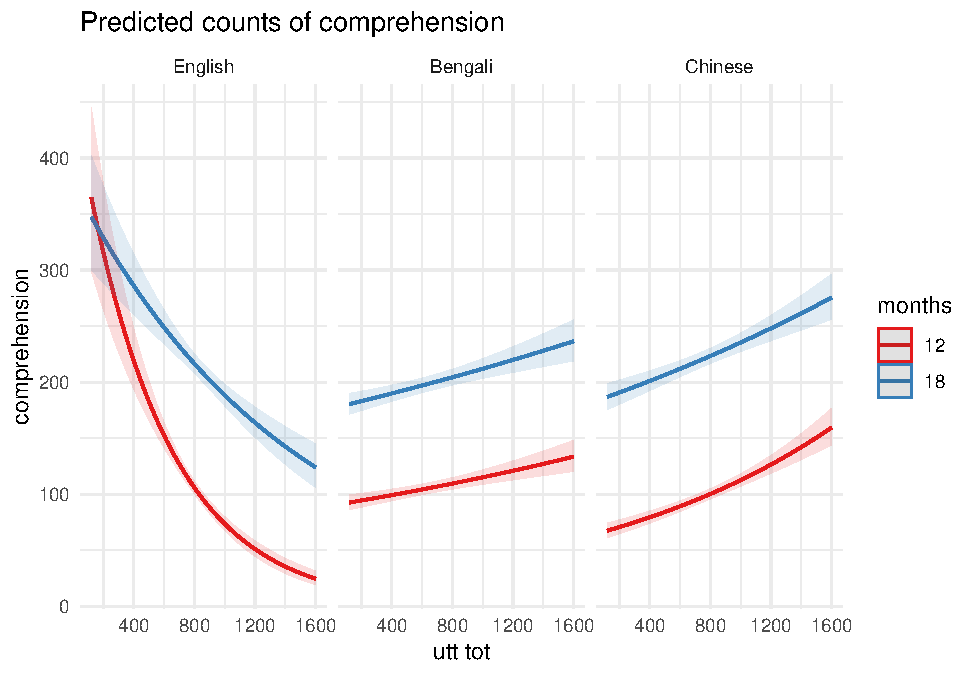
\includegraphics{supplement_files/figure-latex/utt-lm-2-plot-1.pdf}

\hypertarget{contingent-talks}{%
\subsubsection{Contingent talks}\label{contingent-talks}}

\begin{Shaded}
\begin{Highlighting}[]
\NormalTok{ct_lm <-}\StringTok{ }\KeywordTok{glm}\NormalTok{(}
\NormalTok{  comprehension }\OperatorTok{~}
\StringTok{    }\NormalTok{ct_tot }\OperatorTok{*}
\StringTok{    }\NormalTok{months }\OperatorTok{*}
\StringTok{    }\NormalTok{background,}
  \DataTypeTok{data =} \KeywordTok{filter}\NormalTok{(vocab, ct_tot }\OperatorTok{<}\StringTok{ }\DecValTok{30}\NormalTok{),}
  \DataTypeTok{family =} \KeywordTok{poisson}\NormalTok{()}
\NormalTok{)}
\KeywordTok{summary}\NormalTok{(ct_lm)}
\end{Highlighting}
\end{Shaded}

\begin{verbatim}
## 
## Call:
## glm(formula = comprehension ~ ct_tot * months * background, family = poisson(), 
##     data = filter(vocab, ct_tot < 30))
## 
## Deviance Residuals: 
##      Min        1Q    Median        3Q       Max  
## -13.4501   -4.6077   -0.2327    3.4079   19.6808  
## 
## Coefficients:
##                                    Estimate Std. Error z value Pr(>|z|)
## (Intercept)                        4.637232   0.034058 136.157  < 2e-16
## ct_tot                            -0.014368   0.003855  -3.727 0.000194
## months18                           0.633921   0.041849  15.148  < 2e-16
## backgroundBengali                 -0.130032   0.044814  -2.902 0.003713
## backgroundChinese                 -0.314289   0.051969  -6.048 1.47e-09
## ct_tot:months18                    0.028783   0.004487   6.415 1.41e-10
## ct_tot:backgroundBengali           0.053121   0.005997   8.857  < 2e-16
## ct_tot:backgroundChinese           0.051221   0.004907  10.439  < 2e-16
## months18:backgroundBengali         0.104409   0.054990   1.899 0.057603
## months18:backgroundChinese         0.286084   0.062807   4.555 5.24e-06
## ct_tot:months18:backgroundBengali -0.057756   0.007397  -7.808 5.80e-15
## ct_tot:months18:backgroundChinese -0.044388   0.005814  -7.635 2.26e-14
##                                      
## (Intercept)                       ***
## ct_tot                            ***
## months18                          ***
## backgroundBengali                 ** 
## backgroundChinese                 ***
## ct_tot:months18                   ***
## ct_tot:backgroundBengali          ***
## ct_tot:backgroundChinese          ***
## months18:backgroundBengali        .  
## months18:backgroundChinese        ***
## ct_tot:months18:backgroundBengali ***
## ct_tot:months18:backgroundChinese ***
## ---
## Signif. codes:  0 '***' 0.001 '**' 0.01 '*' 0.05 '.' 0.1 ' ' 1
## 
## (Dispersion parameter for poisson family taken to be 1)
## 
##     Null deviance: 6335.5  on 104  degrees of freedom
## Residual deviance: 3804.5  on  93  degrees of freedom
##   (1 observation deleted due to missingness)
## AIC: 4526.8
## 
## Number of Fisher Scoring iterations: 5
\end{verbatim}

\begin{Shaded}
\begin{Highlighting}[]
\KeywordTok{plot_model}\NormalTok{(ct_lm, }\DataTypeTok{type =} \StringTok{"pred"}\NormalTok{, }\DataTypeTok{terms =} \KeywordTok{c}\NormalTok{(}\StringTok{"ct_tot"}\NormalTok{, }\StringTok{"months"}\NormalTok{, }\StringTok{"background"}\NormalTok{))}
\end{Highlighting}
\end{Shaded}

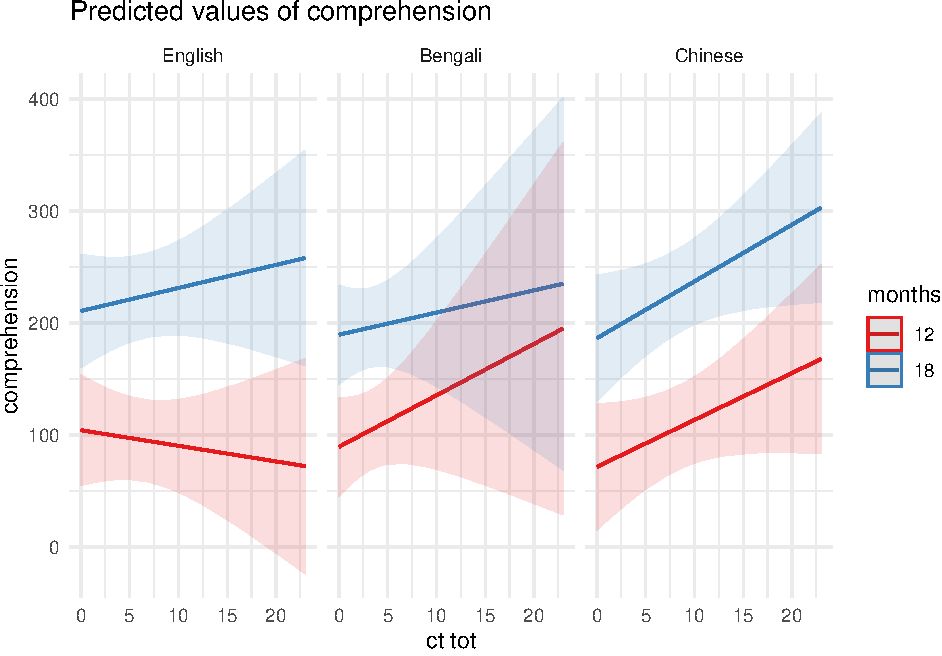
\includegraphics{supplement_files/figure-latex/ct-lm-2-plot-1.pdf}

\hypertarget{production-at-12-and-18-months}{%
\subsection{Production at 12 and 18
months}\label{production-at-12-and-18-months}}

\hypertarget{all-gestures-combined-1}{%
\subsubsection{All gestures combined}\label{all-gestures-combined-1}}

\begin{Shaded}
\begin{Highlighting}[]
\NormalTok{all_gest_prod <-}\StringTok{ }\KeywordTok{glm}\NormalTok{(}
\NormalTok{  production }\OperatorTok{~}
\StringTok{    }\NormalTok{count_tot }\OperatorTok{*}
\StringTok{    }\NormalTok{months }\OperatorTok{*}
\StringTok{    }\NormalTok{background,}
  \DataTypeTok{data =}\NormalTok{ vocab,}
  \DataTypeTok{family =} \KeywordTok{poisson}\NormalTok{()}
\NormalTok{)}
\KeywordTok{summary}\NormalTok{(all_gest_prod)}
\end{Highlighting}
\end{Shaded}

\begin{verbatim}
## 
## Call:
## glm(formula = production ~ count_tot * months * background, family = poisson(), 
##     data = vocab)
## 
## Deviance Residuals: 
##     Min       1Q   Median       3Q      Max  
## -9.4957  -4.2027  -1.2293   0.9099  28.3218  
## 
## Coefficients:
##                                       Estimate Std. Error z value Pr(>|z|)
## (Intercept)                           2.166316   0.098032  22.098  < 2e-16
## count_tot                             0.003990   0.001628   2.451   0.0142
## months18                              1.601423   0.106336  15.060  < 2e-16
## backgroundBengali                     0.106356   0.189875   0.560   0.5754
## backgroundChinese                    -1.270756   0.241938  -5.252 1.50e-07
## count_tot:months18                    0.006925   0.001700   4.074 4.62e-05
## count_tot:backgroundBengali          -0.005035   0.004041  -1.246   0.2127
## count_tot:backgroundChinese           0.006937   0.004082   1.699   0.0892
## months18:backgroundBengali           -0.064505   0.208611  -0.309   0.7572
## months18:backgroundChinese            0.011565   0.256854   0.045   0.9641
## count_tot:months18:backgroundBengali -0.007497   0.004425  -1.694   0.0902
## count_tot:months18:backgroundChinese  0.008679   0.004237   2.048   0.0405
##                                         
## (Intercept)                          ***
## count_tot                            *  
## months18                             ***
## backgroundBengali                       
## backgroundChinese                    ***
## count_tot:months18                   ***
## count_tot:backgroundBengali             
## count_tot:backgroundChinese          .  
## months18:backgroundBengali              
## months18:backgroundChinese              
## count_tot:months18:backgroundBengali .  
## count_tot:months18:backgroundChinese *  
## ---
## Signif. codes:  0 '***' 0.001 '**' 0.01 '*' 0.05 '.' 0.1 ' ' 1
## 
## (Dispersion parameter for poisson family taken to be 1)
## 
##     Null deviance: 6616.0  on 108  degrees of freedom
## Residual deviance: 3247.6  on  97  degrees of freedom
##   (11 observations deleted due to missingness)
## AIC: 3711.3
## 
## Number of Fisher Scoring iterations: 6
\end{verbatim}

\begin{Shaded}
\begin{Highlighting}[]
\KeywordTok{plot_model}\NormalTok{(all_gest_prod, }\DataTypeTok{type =} \StringTok{"pred"}\NormalTok{, }\DataTypeTok{terms =} \KeywordTok{c}\NormalTok{(}\StringTok{"count_tot"}\NormalTok{, }\StringTok{"months"}\NormalTok{, }\StringTok{"background"}\NormalTok{))}
\end{Highlighting}
\end{Shaded}

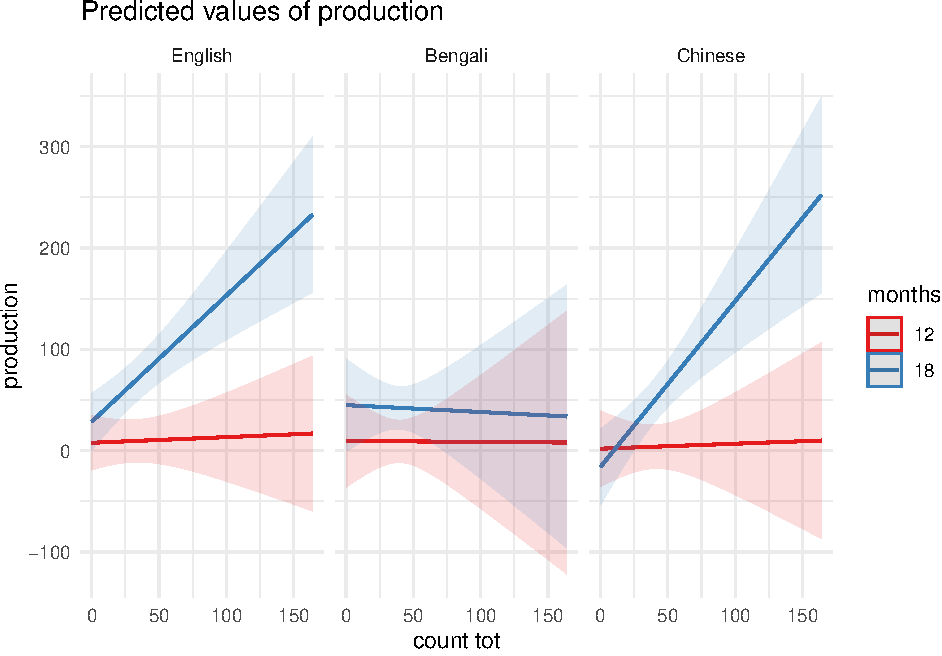
\includegraphics{supplement_files/figure-latex/all-gest-lm-2-undsay-plot-1.pdf}

\hypertarget{hogs-point}{%
\subsubsection{HoGs + point}\label{hogs-point}}

\begin{Shaded}
\begin{Highlighting}[]
\NormalTok{hgp_prod <-}\StringTok{ }\KeywordTok{glm}\NormalTok{(}
\NormalTok{  production }\OperatorTok{~}
\StringTok{    }\NormalTok{hgp_tot }\OperatorTok{*}
\StringTok{    }\NormalTok{months }\OperatorTok{*}
\StringTok{    }\NormalTok{background,}
  \DataTypeTok{data =}\NormalTok{ vocab,}
  \KeywordTok{poisson}\NormalTok{()}
\NormalTok{)}
\KeywordTok{summary}\NormalTok{(hgp_prod)}
\end{Highlighting}
\end{Shaded}

\begin{verbatim}
## 
## Call:
## glm(formula = production ~ hgp_tot * months * background, family = poisson(), 
##     data = vocab)
## 
## Deviance Residuals: 
##      Min        1Q    Median        3Q       Max  
## -10.1715   -4.3463   -1.2156    0.8963   28.5549  
## 
## Coefficients:
##                                     Estimate Std. Error z value Pr(>|z|)
## (Intercept)                         2.245524   0.089517  25.085  < 2e-16
## hgp_tot                             0.002311   0.001714   1.348   0.1776
## months18                            1.615544   0.097321  16.600  < 2e-16
## backgroundBengali                   0.011640   0.167801   0.069   0.9447
## backgroundChinese                  -1.137042   0.209942  -5.416 6.09e-08
## hgp_tot:months18                    0.008156   0.001776   4.592 4.38e-06
## hgp_tot:backgroundBengali          -0.003219   0.004646  -0.693   0.4883
## hgp_tot:backgroundChinese           0.005629   0.004230   1.331   0.1833
## months18:backgroundBengali          0.003230   0.184145   0.018   0.9860
## months18:backgroundChinese          0.158991   0.223274   0.712   0.4764
## hgp_tot:months18:backgroundBengali -0.011967   0.005105  -2.344   0.0191
## hgp_tot:months18:backgroundChinese  0.007893   0.004380   1.802   0.0715
##                                       
## (Intercept)                        ***
## hgp_tot                               
## months18                           ***
## backgroundBengali                     
## backgroundChinese                  ***
## hgp_tot:months18                   ***
## hgp_tot:backgroundBengali             
## hgp_tot:backgroundChinese             
## months18:backgroundBengali            
## months18:backgroundChinese            
## hgp_tot:months18:backgroundBengali *  
## hgp_tot:months18:backgroundChinese .  
## ---
## Signif. codes:  0 '***' 0.001 '**' 0.01 '*' 0.05 '.' 0.1 ' ' 1
## 
## (Dispersion parameter for poisson family taken to be 1)
## 
##     Null deviance: 6616.0  on 108  degrees of freedom
## Residual deviance: 3391.2  on  97  degrees of freedom
##   (11 observations deleted due to missingness)
## AIC: 3854.9
## 
## Number of Fisher Scoring iterations: 6
\end{verbatim}

\begin{Shaded}
\begin{Highlighting}[]
\KeywordTok{plot_model}\NormalTok{(hgp_prod, }\DataTypeTok{type =} \StringTok{"pred"}\NormalTok{, }\DataTypeTok{terms =} \KeywordTok{c}\NormalTok{(}\StringTok{"hgp_tot"}\NormalTok{, }\StringTok{"months"}\NormalTok{, }\StringTok{"background"}\NormalTok{))}
\end{Highlighting}
\end{Shaded}

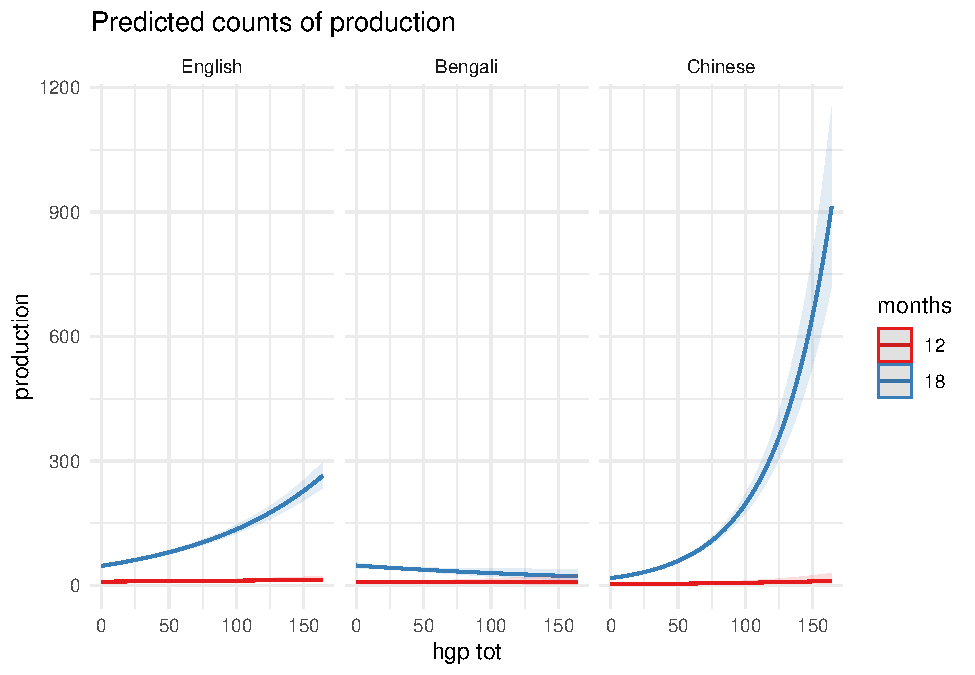
\includegraphics{supplement_files/figure-latex/hgp-lm-2-undsay-plot-1.pdf}

\hypertarget{reaches-2}{%
\subsubsection{Reaches}\label{reaches-2}}

\begin{Shaded}
\begin{Highlighting}[]
\NormalTok{reach_prod <-}\StringTok{ }\KeywordTok{glm}\NormalTok{(}
\NormalTok{  production }\OperatorTok{~}
\StringTok{    }\NormalTok{reach_tot }\OperatorTok{*}
\StringTok{    }\NormalTok{months }\OperatorTok{*}
\StringTok{    }\NormalTok{background,}
  \DataTypeTok{data =}\NormalTok{ vocab,}
  \DataTypeTok{family =} \KeywordTok{poisson}\NormalTok{()}
\NormalTok{)}
\KeywordTok{summary}\NormalTok{(reach_prod)}
\end{Highlighting}
\end{Shaded}

\begin{verbatim}
## 
## Call:
## glm(formula = production ~ reach_tot * months * background, family = poisson(), 
##     data = vocab)
## 
## Deviance Residuals: 
##     Min       1Q   Median       3Q      Max  
## -11.152   -4.326   -1.274    1.089   27.720  
## 
## Coefficients:
##                                      Estimate Std. Error z value Pr(>|z|)
## (Intercept)                           1.77394    0.12626  14.050  < 2e-16
## reach_tot                             0.06271    0.01005   6.239 4.40e-10
## months18                              2.57343    0.13262  19.405  < 2e-16
## backgroundBengali                     0.49872    0.19502   2.557 0.010549
## backgroundChinese                    -1.36596    0.30542  -4.472 7.73e-06
## reach_tot:months18                   -0.07546    0.01097  -6.877 6.11e-12
## reach_tot:backgroundBengali          -0.06637    0.01531  -4.336 1.45e-05
## reach_tot:backgroundChinese           0.03494    0.02410   1.450 0.147099
## months18:backgroundBengali           -1.29841    0.21214  -6.121 9.32e-10
## months18:backgroundChinese           -0.15125    0.31853  -0.475 0.634915
## reach_tot:months18:backgroundBengali  0.09620    0.01679   5.729 1.01e-08
## reach_tot:months18:backgroundChinese  0.08389    0.02529   3.317 0.000909
##                                         
## (Intercept)                          ***
## reach_tot                            ***
## months18                             ***
## backgroundBengali                    *  
## backgroundChinese                    ***
## reach_tot:months18                   ***
## reach_tot:backgroundBengali          ***
## reach_tot:backgroundChinese             
## months18:backgroundBengali           ***
## months18:backgroundChinese              
## reach_tot:months18:backgroundBengali ***
## reach_tot:months18:backgroundChinese ***
## ---
## Signif. codes:  0 '***' 0.001 '**' 0.01 '*' 0.05 '.' 0.1 ' ' 1
## 
## (Dispersion parameter for poisson family taken to be 1)
## 
##     Null deviance: 6616.0  on 108  degrees of freedom
## Residual deviance: 3934.9  on  97  degrees of freedom
##   (11 observations deleted due to missingness)
## AIC: 4398.6
## 
## Number of Fisher Scoring iterations: 6
\end{verbatim}

\begin{Shaded}
\begin{Highlighting}[]
\KeywordTok{plot_model}\NormalTok{(reach_prod, }\DataTypeTok{type =} \StringTok{"pred"}\NormalTok{, }\DataTypeTok{terms =} \KeywordTok{c}\NormalTok{(}\StringTok{"reach_tot"}\NormalTok{, }\StringTok{"months"}\NormalTok{, }\StringTok{"background"}\NormalTok{))}
\end{Highlighting}
\end{Shaded}

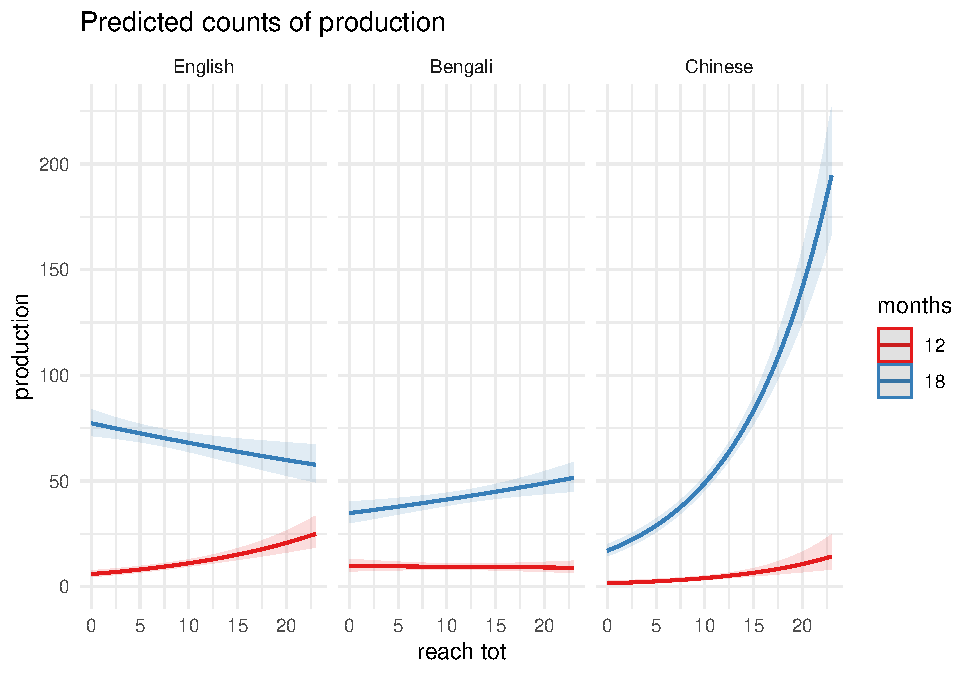
\includegraphics{supplement_files/figure-latex/reach-lm-2-undsay-plot-1.pdf}

\hypertarget{maternal-utterances-1}{%
\subsubsection{Maternal utterances}\label{maternal-utterances-1}}

\begin{Shaded}
\begin{Highlighting}[]
\NormalTok{utt_prod <-}\StringTok{ }\KeywordTok{glm}\NormalTok{(}
\NormalTok{  production }\OperatorTok{~}
\StringTok{    }\NormalTok{utt_tot }\OperatorTok{*}
\StringTok{    }\NormalTok{months }\OperatorTok{*}
\StringTok{    }\NormalTok{background,}
  \DataTypeTok{data =}\NormalTok{ vocab,}
  \DataTypeTok{family =} \KeywordTok{poisson}\NormalTok{()}
\NormalTok{)}
\KeywordTok{summary}\NormalTok{(utt_prod)}
\end{Highlighting}
\end{Shaded}

\begin{verbatim}
## 
## Call:
## glm(formula = production ~ utt_tot * months * background, family = poisson(), 
##     data = vocab)
## 
## Deviance Residuals: 
##     Min       1Q   Median       3Q      Max  
## -15.241   -3.563   -1.206    1.294   21.551  
## 
## Coefficients:
##                                      Estimate Std. Error z value Pr(>|z|)
## (Intercept)                         1.3192300  0.4676905   2.821  0.00479
## utt_tot                             0.0006349  0.0005199   1.221  0.22202
## months18                            2.2536527  0.5013805   4.495 6.96e-06
## backgroundBengali                   0.2990578  0.4911280   0.609  0.54258
## backgroundChinese                  -0.3297520  0.5434137  -0.607  0.54397
## utt_tot:months18                   -0.0002767  0.0005571  -0.497  0.61938
## utt_tot:backgroundBengali           0.0002044  0.0005441   0.376  0.70713
## utt_tot:backgroundChinese          -0.0001612  0.0006045  -0.267  0.78978
## months18:backgroundBengali         -1.2230964  0.5287705  -2.313  0.02072
## months18:backgroundChinese          0.4936444  0.5778999   0.854  0.39299
## utt_tot:months18:backgroundBengali  0.0009362  0.0005839   1.603  0.10887
## utt_tot:months18:backgroundChinese -0.0000419  0.0006432  -0.065  0.94806
##                                       
## (Intercept)                        ** 
## utt_tot                               
## months18                           ***
## backgroundBengali                     
## backgroundChinese                     
## utt_tot:months18                      
## utt_tot:backgroundBengali             
## utt_tot:backgroundChinese             
## months18:backgroundBengali         *  
## months18:backgroundChinese            
## utt_tot:months18:backgroundBengali    
## utt_tot:months18:backgroundChinese    
## ---
## Signif. codes:  0 '***' 0.001 '**' 0.01 '*' 0.05 '.' 0.1 ' ' 1
## 
## (Dispersion parameter for poisson family taken to be 1)
## 
##     Null deviance: 5308.0  on 98  degrees of freedom
## Residual deviance: 3069.1  on 87  degrees of freedom
##   (21 observations deleted due to missingness)
## AIC: 3480.5
## 
## Number of Fisher Scoring iterations: 6
\end{verbatim}

\begin{Shaded}
\begin{Highlighting}[]
\KeywordTok{plot_model}\NormalTok{(utt_prod, }\DataTypeTok{type =} \StringTok{"pred"}\NormalTok{, }\DataTypeTok{terms =} \KeywordTok{c}\NormalTok{(}\StringTok{"utt_tot"}\NormalTok{, }\StringTok{"months"}\NormalTok{, }\StringTok{"background"}\NormalTok{))}
\end{Highlighting}
\end{Shaded}

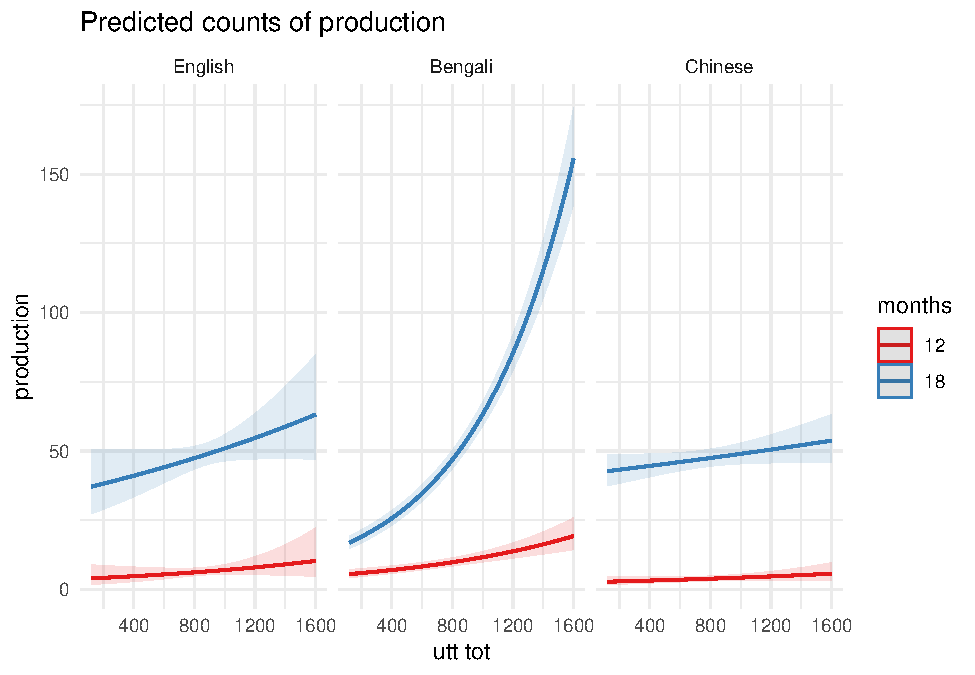
\includegraphics{supplement_files/figure-latex/utt-lm-2-undsay-plot-1.pdf}

\hypertarget{contingent-talks-1}{%
\subsubsection{Contingent talks}\label{contingent-talks-1}}

\begin{Shaded}
\begin{Highlighting}[]
\NormalTok{ct_prod <-}\StringTok{ }\KeywordTok{glm}\NormalTok{(}
\NormalTok{  production }\OperatorTok{~}
\StringTok{    }\NormalTok{ct_tot }\OperatorTok{*}
\StringTok{    }\NormalTok{months }\OperatorTok{*}
\StringTok{    }\NormalTok{background,}
  \DataTypeTok{data =} \KeywordTok{filter}\NormalTok{(vocab, ct_tot }\OperatorTok{<}\StringTok{ }\DecValTok{30}\NormalTok{),}
  \DataTypeTok{family =} \KeywordTok{poisson}\NormalTok{()}
\NormalTok{)}
\KeywordTok{summary}\NormalTok{(ct_prod)}
\end{Highlighting}
\end{Shaded}

\begin{verbatim}
## 
## Call:
## glm(formula = production ~ ct_tot * months * background, family = poisson(), 
##     data = filter(vocab, ct_tot < 30))
## 
## Deviance Residuals: 
##     Min       1Q   Median       3Q      Max  
## -10.399   -3.871   -1.082    1.232   19.069  
## 
## Coefficients:
##                                    Estimate Std. Error z value Pr(>|z|)
## (Intercept)                        1.964853   0.116021  16.935  < 2e-16
## ct_tot                             0.045305   0.009572   4.733 2.21e-06
## months18                           1.530771   0.127526  12.004  < 2e-16
## backgroundBengali                 -0.140679   0.157079  -0.896  0.37047
## backgroundChinese                 -1.389104   0.264167  -5.258 1.45e-07
## ct_tot:months18                    0.026242   0.010293   2.550  0.01078
## ct_tot:backgroundBengali           0.049489   0.016404   3.017  0.00255
## ct_tot:backgroundChinese           0.026008   0.018783   1.385  0.16617
## months18:backgroundBengali        -0.487944   0.175556  -2.779  0.00545
## months18:backgroundChinese         1.348792   0.275822   4.890 1.01e-06
## ct_tot:months18:backgroundBengali  0.047711   0.017752   2.688  0.00719
## ct_tot:months18:backgroundChinese -0.048643   0.019651  -2.475  0.01331
##                                      
## (Intercept)                       ***
## ct_tot                            ***
## months18                          ***
## backgroundBengali                    
## backgroundChinese                 ***
## ct_tot:months18                   *  
## ct_tot:backgroundBengali          ** 
## ct_tot:backgroundChinese             
## months18:backgroundBengali        ** 
## months18:backgroundChinese        ***
## ct_tot:months18:backgroundBengali ** 
## ct_tot:months18:backgroundChinese *  
## ---
## Signif. codes:  0 '***' 0.001 '**' 0.01 '*' 0.05 '.' 0.1 ' ' 1
## 
## (Dispersion parameter for poisson family taken to be 1)
## 
##     Null deviance: 6123.3  on 104  degrees of freedom
## Residual deviance: 2765.6  on  93  degrees of freedom
##   (1 observation deleted due to missingness)
## AIC: 3209.7
## 
## Number of Fisher Scoring iterations: 6
\end{verbatim}

\begin{Shaded}
\begin{Highlighting}[]
\KeywordTok{plot_model}\NormalTok{(ct_prod, }\DataTypeTok{type =} \StringTok{"pred"}\NormalTok{, }\DataTypeTok{terms =} \KeywordTok{c}\NormalTok{(}\StringTok{"ct_tot"}\NormalTok{, }\StringTok{"months"}\NormalTok{, }\StringTok{"background"}\NormalTok{))}
\end{Highlighting}
\end{Shaded}

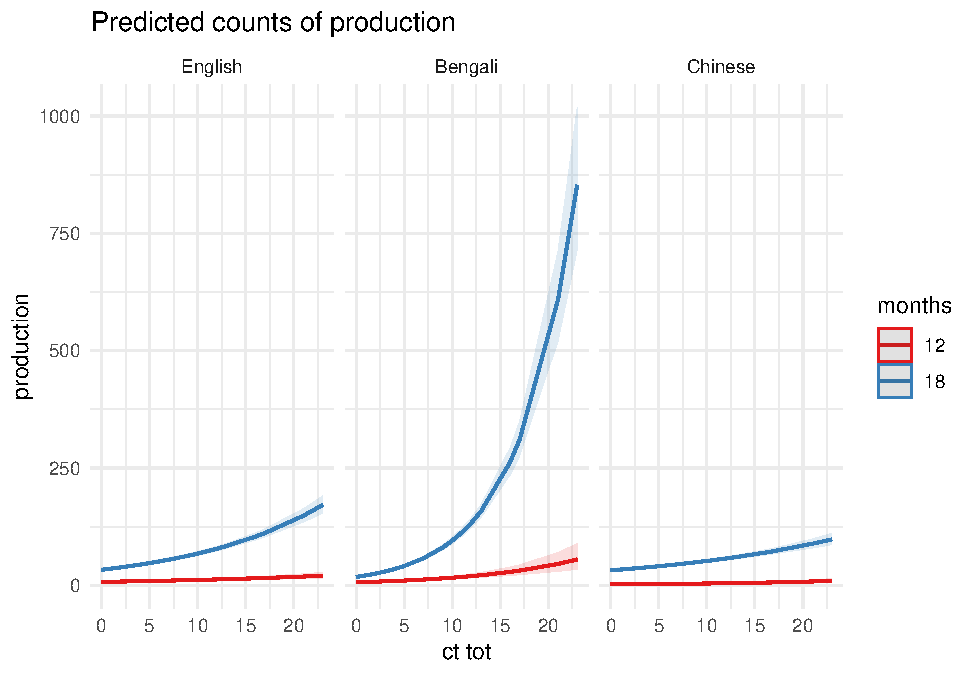
\includegraphics{supplement_files/figure-latex/ct-lm-2-undsay-plot-1.pdf}

\newpage

\hypertarget{number-of-observations}{%
\section{Number of observations}\label{number-of-observations}}

The following sections report the number of observations (excluding NAs)
used in the models above.

\hypertarget{analysis-1a}{%
\subsection{Analysis 1a}\label{analysis-1a}}

\hypertarget{reaches-3}{%
\subsubsection{Reaches}\label{reaches-3}}

\begin{Shaded}
\begin{Highlighting}[]
\NormalTok{reach_tot }\OperatorTok
\StringTok{  }\KeywordTok{group_by}\NormalTok{(back_o, months) }\OperatorTok
\StringTok{  }\KeywordTok{na.omit}\NormalTok{() }\OperatorTok
\StringTok{  }\KeywordTok{summarise}\NormalTok{(}\DataTypeTok{n =} \KeywordTok{n}\NormalTok{())}
\end{Highlighting}
\end{Shaded}

\begin{verbatim}
## # A tibble: 9 x 3
## # Groups:   back_o [3]
##   back_o  months     n
##   <ord>    <dbl> <int>
## 1 English     10    19
## 2 English     11    19
## 3 English     12    18
## 4 Bengali     10    20
## 5 Bengali     11    19
## 6 Bengali     12    19
## 7 Chinese     10    18
## 8 Chinese     11    19
## 9 Chinese     12    20
\end{verbatim}

\hypertarget{hogs-1}{%
\subsubsection{HoGs}\label{hogs-1}}

\begin{Shaded}
\begin{Highlighting}[]
\NormalTok{hg_tot }\OperatorTok
\StringTok{  }\KeywordTok{group_by}\NormalTok{(back_o, months) }\OperatorTok
\StringTok{  }\KeywordTok{na.omit}\NormalTok{() }\OperatorTok
\StringTok{  }\KeywordTok{summarise}\NormalTok{(}\DataTypeTok{n =} \KeywordTok{n}\NormalTok{())}
\end{Highlighting}
\end{Shaded}

\begin{verbatim}
## # A tibble: 9 x 3
## # Groups:   back_o [3]
##   back_o  months     n
##   <ord>    <dbl> <int>
## 1 English     10    19
## 2 English     11    19
## 3 English     12    18
## 4 Bengali     10    20
## 5 Bengali     11    19
## 6 Bengali     12    19
## 7 Chinese     10    18
## 8 Chinese     11    19
## 9 Chinese     12    20
\end{verbatim}

\hypertarget{points}{%
\subsubsection{Points}\label{points}}

\begin{Shaded}
\begin{Highlighting}[]
\NormalTok{point_tot }\OperatorTok
\StringTok{  }\KeywordTok{group_by}\NormalTok{(back_o, months) }\OperatorTok
\StringTok{  }\KeywordTok{na.omit}\NormalTok{() }\OperatorTok
\StringTok{  }\KeywordTok{summarise}\NormalTok{(}\DataTypeTok{n =} \KeywordTok{n}\NormalTok{())}
\end{Highlighting}
\end{Shaded}

\begin{verbatim}
## # A tibble: 9 x 3
## # Groups:   back_o [3]
##   back_o  months     n
##   <ord>    <dbl> <int>
## 1 English     10    19
## 2 English     11    19
## 3 English     12    18
## 4 Bengali     10    20
## 5 Bengali     11    19
## 6 Bengali     12    19
## 7 Chinese     10    18
## 8 Chinese     11    19
## 9 Chinese     12    20
\end{verbatim}

\hypertarget{analysis-1c}{%
\subsection{Analysis 1c}\label{analysis-1c}}

\hypertarget{maternal-utterances-2}{%
\subsubsection{Maternal utterances}\label{maternal-utterances-2}}

\begin{Shaded}
\begin{Highlighting}[]
\NormalTok{utterances_tot }\OperatorTok
\StringTok{  }\KeywordTok{group_by}\NormalTok{(back_o, months) }\OperatorTok
\StringTok{  }\KeywordTok{na.omit}\NormalTok{() }\OperatorTok
\StringTok{  }\KeywordTok{summarise}\NormalTok{(}\DataTypeTok{n =} \KeywordTok{n}\NormalTok{())}
\end{Highlighting}
\end{Shaded}

\begin{verbatim}
## # A tibble: 9 x 3
## # Groups:   back_o [3]
##   back_o  months     n
##   <ord>    <dbl> <int>
## 1 English     10    17
## 2 English     11    18
## 3 English     12    16
## 4 Bengali     10    20
## 5 Bengali     11    19
## 6 Bengali     12    18
## 7 Chinese     10    19
## 8 Chinese     11    20
## 9 Chinese     12    20
\end{verbatim}

\hypertarget{maternal-cts}{%
\subsubsection{Maternal CTs}\label{maternal-cts}}

\begin{Shaded}
\begin{Highlighting}[]
\NormalTok{all_tot }\OperatorTok
\StringTok{  }\KeywordTok{group_by}\NormalTok{(back_o, months) }\OperatorTok
\StringTok{  }\KeywordTok{na.omit}\NormalTok{() }\OperatorTok
\StringTok{  }\KeywordTok{summarise}\NormalTok{(}\DataTypeTok{n =} \KeywordTok{n}\NormalTok{())}
\end{Highlighting}
\end{Shaded}

\begin{verbatim}
## # A tibble: 9 x 3
## # Groups:   back_o [3]
##   back_o  months     n
##   <ord>    <dbl> <int>
## 1 English     10    19
## 2 English     11    19
## 3 English     12    18
## 4 Bengali     10    20
## 5 Bengali     11    19
## 6 Bengali     12    19
## 7 Chinese     10    18
## 8 Chinese     11    19
## 9 Chinese     12    20
\end{verbatim}

\hypertarget{analysis-1c-1}{%
\subsection{Analysis 1c}\label{analysis-1c-1}}

\hypertarget{reaches-4}{%
\subsubsection{Reaches}\label{reaches-4}}

\begin{Shaded}
\begin{Highlighting}[]
\NormalTok{reach_point_lead }\OperatorTok
\StringTok{  }\KeywordTok{group_by}\NormalTok{(back_o) }\OperatorTok
\StringTok{  }\KeywordTok{na.omit}\NormalTok{() }\OperatorTok
\StringTok{  }\KeywordTok{summarise}\NormalTok{(}\DataTypeTok{n =} \KeywordTok{n}\NormalTok{())}
\end{Highlighting}
\end{Shaded}

\begin{verbatim}
## # A tibble: 3 x 2
##   back_o      n
##   <ord>   <int>
## 1 English    37
## 2 Bengali    38
## 3 Chinese    37
\end{verbatim}

\hypertarget{hogs-2}{%
\subsubsection{HoGs}\label{hogs-2}}

\begin{Shaded}
\begin{Highlighting}[]
\NormalTok{hg_point_lead }\OperatorTok
\StringTok{  }\KeywordTok{group_by}\NormalTok{(back_o) }\OperatorTok
\StringTok{  }\KeywordTok{na.omit}\NormalTok{() }\OperatorTok
\StringTok{  }\KeywordTok{summarise}\NormalTok{(}\DataTypeTok{n =} \KeywordTok{n}\NormalTok{())}
\end{Highlighting}
\end{Shaded}

\begin{verbatim}
## # A tibble: 3 x 2
##   back_o      n
##   <ord>   <int>
## 1 English    37
## 2 Bengali    38
## 3 Chinese    37
\end{verbatim}

\hypertarget{analysis-2}{%
\subsection{Analysis 2}\label{analysis-2}}

The counts apply both to the comprehension and production analyses.

\begin{Shaded}
\begin{Highlighting}[]
\NormalTok{vocab }\OperatorTok
\StringTok{  }\KeywordTok{group_by}\NormalTok{(background) }\OperatorTok
\StringTok{  }\KeywordTok{na.omit}\NormalTok{() }\OperatorTok
\StringTok{  }\KeywordTok{summarise}\NormalTok{(}\DataTypeTok{n =} \KeywordTok{n}\NormalTok{())}
\end{Highlighting}
\end{Shaded}

\begin{verbatim}
## # A tibble: 3 x 2
##   background     n
##   <fct>      <int>
## 1 English       25
## 2 Bengali       34
## 3 Chinese       34
\end{verbatim}

\hypertarget{r-session}{%
\section{R session}\label{r-session}}

\begin{Shaded}
\begin{Highlighting}[]
\KeywordTok{sessionInfo}\NormalTok{()}
\end{Highlighting}
\end{Shaded}

\begin{verbatim}
## R version 3.5.3 (2019-03-11)
## Platform: x86_64-apple-darwin15.6.0 (64-bit)
## Running under: macOS Mojave 10.14.5
## 
## Matrix products: default
## BLAS: /Library/Frameworks/R.framework/Versions/3.5/Resources/lib/libRblas.0.dylib
## LAPACK: /Library/Frameworks/R.framework/Versions/3.5/Resources/lib/libRlapack.dylib
## 
## locale:
## [1] en_GB.UTF-8/en_GB.UTF-8/en_GB.UTF-8/C/en_GB.UTF-8/en_GB.UTF-8
## 
## attached base packages:
## [1] stats     graphics  grDevices utils     datasets  methods   base     
## 
## other attached packages:
##  [1] sjPlot_2.6.3      simr_1.0.5        effects_4.1-1    
##  [4] carData_3.0-2     lmerTest_3.1-0    lme4_1.1-21      
##  [7] Matrix_1.2-17     tidymv_2.2.0      itsadug_2.3      
## [10] plotfunctions_1.3 mgcv_1.8-28       nlme_3.1-140     
## [13] forcats_0.4.0     stringr_1.4.0     dplyr_0.8.2      
## [16] purrr_0.3.2       readr_1.3.1       tidyr_0.8.3      
## [19] tibble_2.1.3      ggplot2_3.2.0     tidyverse_1.2.1  
## [22] MASS_7.3-51.4    
## 
## loaded via a namespace (and not attached):
##  [1] TH.data_1.0-10      minqa_1.2.4         colorspace_1.4-1   
##  [4] rio_0.5.16          sjlabelled_1.1.0    snakecase_0.11.0   
##  [7] estimability_1.3    rstudioapi_0.10     glmmTMB_0.2.3      
## [10] mvtnorm_1.0-11      lubridate_1.7.4     xml2_1.2.0         
## [13] codetools_0.2-16    splines_3.5.3       mnormt_1.5-5       
## [16] knitr_1.23          sjmisc_2.8.1        jsonlite_1.6       
## [19] nloptr_1.2.1        ggeffects_0.11.0    pbkrtest_0.4-7     
## [22] broom_0.5.2         binom_1.1-1         compiler_3.5.3     
## [25] httr_1.4.0          sjstats_0.17.5      emmeans_1.3.5.1    
## [28] backports_1.1.4     assertthat_0.2.1    lazyeval_0.2.2     
## [31] survey_3.36         cli_1.1.0           htmltools_0.3.6    
## [34] tools_3.5.3         coda_0.19-2         gtable_0.3.0       
## [37] glue_1.3.1          Rcpp_1.0.1          cellranger_1.1.0   
## [40] iterators_1.0.10    psych_1.8.12        insight_0.4.0      
## [43] xfun_0.8            openxlsx_4.1.0.1    rvest_0.3.4        
## [46] zoo_1.8-6           scales_1.0.0        hms_0.4.2          
## [49] parallel_3.5.3      sandwich_2.5-1      RColorBrewer_1.1-2 
## [52] TMB_1.7.15          yaml_2.2.0          curl_3.3           
## [55] stringi_1.4.3       bayestestR_0.2.2    plotrix_3.7-6      
## [58] boot_1.3-22         zip_2.0.3           rlang_0.4.0        
## [61] pkgconfig_2.0.2     evaluate_0.14       lattice_0.20-38    
## [64] labeling_0.3        tidyselect_0.2.5    plyr_1.8.4         
## [67] magrittr_1.5        R6_2.4.0            generics_0.0.2     
## [70] multcomp_1.4-10     RLRsim_3.1-3        DBI_1.0.0          
## [73] pillar_1.4.2        haven_2.1.0         foreign_0.8-71     
## [76] withr_2.1.2         survival_2.44-1.1   abind_1.4-5        
## [79] nnet_7.3-12         performance_0.2.0   modelr_0.1.4       
## [82] crayon_1.3.4        car_3.0-3           rmarkdown_1.13     
## [85] grid_3.5.3          readxl_1.3.1        data.table_1.12.2  
## [88] digest_0.6.19       xtable_1.8-4        numDeriv_2016.8-1.1
## [91] munsell_0.5.0       mitools_2.4
\end{verbatim}


\end{document}
